\batchmode
\documentclass[a4paper]{book}
\usepackage{makeidx}
\usepackage{natbib}
\usepackage{graphicx}
\usepackage{multicol}
\usepackage{float}
\usepackage{listings}
\usepackage{color}
\usepackage{ifthen}
\usepackage[table]{xcolor}
\usepackage{textcomp}
\usepackage{alltt}
\usepackage[utf8]{inputenc}
\usepackage{mathptmx}
\usepackage[scaled=.90]{helvet}
\usepackage{courier}
\usepackage{sectsty}
\usepackage[titles]{tocloft}
\usepackage{doxygen}
\lstset{language=C++,inputencoding=utf8,basicstyle=\footnotesize,breaklines=true,breakatwhitespace=true,tabsize=8,numbers=left }
\makeindex
\setcounter{tocdepth}{3}
\renewcommand{\footrulewidth}{0.4pt}
\renewcommand{\familydefault}{\sfdefault}
\hfuzz=15pt
\setlength{\emergencystretch}{15pt}
\hbadness=750
\tolerance=750
\begin{document}
\begin{titlepage}
\vspace*{7cm}
\begin{center}
{\Large hardware\-\_\-interface }\\
\vspace*{1cm}
{\large \-Generated by Doxygen 1.7.6.1}\\
\vspace*{0.5cm}
{\small Fri Feb 15 2013 10:35:15}\\
\end{center}
\end{titlepage}
\clearemptydoublepage
\pagenumbering{roman}
\tableofcontents
\clearemptydoublepage
\pagenumbering{arabic}
\chapter{\-Namespace \-Index}
\section{\-Namespace \-List}
\-Here is a list of all namespaces with brief descriptions\-:\begin{DoxyCompactList}
\item\contentsline{section}{{\bf controller\-\_\-interface} }{\pageref{namespacecontroller__interface}}{}
\end{DoxyCompactList}

\chapter{\-Class \-Index}
\section{\-Class \-Hierarchy}
\-This inheritance list is sorted roughly, but not completely, alphabetically\-:\begin{DoxyCompactList}
\item \contentsline{section}{controller\-\_\-interface\-:\-:\-Controller\-Base}{\pageref{classcontroller__interface_1_1ControllerBase}}{}
\begin{DoxyCompactList}
\item \contentsline{section}{controller\-\_\-interface\-:\-:\-Controller$<$ \-T $>$}{\pageref{classcontroller__interface_1_1Controller}}{}
\end{DoxyCompactList}
\end{DoxyCompactList}

\chapter{\-Class \-Index}
\section{\-Class \-List}
\-Here are the classes, structs, unions and interfaces with brief descriptions\-:\begin{DoxyCompactList}
\item\contentsline{section}{{\bf controller\-\_\-interface\-::\-Controller$<$ T $>$} \\*\-Controller with a specific hardware interface }{\pageref{classcontroller__interface_1_1Controller}}{}
\item\contentsline{section}{{\bf controller\-\_\-interface\-::\-Controller\-Base} \\*\-Abstract \-Controller \-Interface }{\pageref{classcontroller__interface_1_1ControllerBase}}{}
\end{DoxyCompactList}

\chapter{\-File \-Index}
\section{\-File \-List}
\-Here is a list of all files with brief descriptions\-:\begin{DoxyCompactList}
\item\contentsline{section}{{\bf \-\_\-\-\_\-init\-\_\-\-\_\-.\-py} }{\pageref{____init_____8py}}{}
\item\contentsline{section}{{\bf controller\-\_\-loader.\-h} }{\pageref{controller__loader_8h}}{}
\item\contentsline{section}{{\bf controller\-\_\-loader\-\_\-interface.\-h} }{\pageref{controller__loader__interface_8h}}{}
\item\contentsline{section}{{\bf controller\-\_\-manager.\-cpp} }{\pageref{controller__manager_8cpp}}{}
\item\contentsline{section}{{\bf controller\-\_\-manager.\-h} }{\pageref{controller__manager_8h}}{}
\item\contentsline{section}{{\bf controller\-\_\-manager\-\_\-interface.\-py} }{\pageref{controller__manager__interface_8py}}{}
\item\contentsline{section}{{\bf controller\-\_\-spec.\-h} }{\pageref{controller__spec_8h}}{}
\end{DoxyCompactList}

\chapter{\-Namespace \-Documentation}
\section{hardware\-\_\-interface \-Namespace \-Reference}
\label{namespacehardware__interface}\index{hardware\-\_\-interface@{hardware\-\_\-interface}}
\subsection*{\-Classes}
\begin{DoxyCompactItemize}
\item 
struct {\bf \-Controller\-Info}
\begin{DoxyCompactList}\small\item\em \-Controller \-Information. \end{DoxyCompactList}\item 
class {\bf \-Effort\-Joint\-Interface}
\begin{DoxyCompactList}\small\item\em \doxyref{\-Joint\-Command\-Interface}{p.}{classhardware__interface_1_1JointCommandInterface} for commanding effort-\/based joints \end{DoxyCompactList}\item 
class {\bf \-Hardware\-Interface}
\begin{DoxyCompactList}\small\item\em \-Abstract \-Hardware \-Interface. \end{DoxyCompactList}\item 
class {\bf \-Hardware\-Interface\-Exception}
\begin{DoxyCompactList}\small\item\em \-An exception related to a \doxyref{\-Hardware\-Interface}{p.}{classhardware__interface_1_1HardwareInterface}. \end{DoxyCompactList}\item 
class {\bf \-Joint\-Command\-Interface}
\begin{DoxyCompactList}\small\item\em \-Hardware interface to support commanding an array of joints. \end{DoxyCompactList}\item 
class {\bf \-Joint\-Handle}
\begin{DoxyCompactList}\small\item\em \-A handle used to read and command a single joint. \end{DoxyCompactList}\item 
class {\bf \-Joint\-State\-Handle}
\begin{DoxyCompactList}\small\item\em \-A handle used to read the state of a single joint. \end{DoxyCompactList}\item 
class {\bf \-Joint\-State\-Interface}
\begin{DoxyCompactList}\small\item\em \-Hardware interface to support reading the state of an array of joints. \end{DoxyCompactList}\item 
class {\bf \-Position\-Joint\-Interface}
\begin{DoxyCompactList}\small\item\em \doxyref{\-Joint\-Command\-Interface}{p.}{classhardware__interface_1_1JointCommandInterface} for commanding position-\/based joints \end{DoxyCompactList}\item 
class {\bf \-Robot\-H\-W}
\begin{DoxyCompactList}\small\item\em \-Robot \-Hardware \-Interface and \-Resource \-Manager. \end{DoxyCompactList}\item 
class {\bf \-Velocity\-Joint\-Interface}
\begin{DoxyCompactList}\small\item\em \doxyref{\-Joint\-Command\-Interface}{p.}{classhardware__interface_1_1JointCommandInterface} for commanding velocity-\/based joints \end{DoxyCompactList}\end{DoxyCompactItemize}

\chapter{\-Class \-Documentation}
\section{hardware\-\_\-interface\-:\-:\-Controller\-Info \-Struct \-Reference}
\label{structhardware__interface_1_1ControllerInfo}\index{hardware\-\_\-interface\-::\-Controller\-Info@{hardware\-\_\-interface\-::\-Controller\-Info}}


\-Controller \-Information.  




{\ttfamily \#include $<$controller\-\_\-info.\-h$>$}

\subsection*{\-Public \-Attributes}
\begin{DoxyCompactItemize}
\item 
std\-::string {\bf hardware\-\_\-interface}
\item 
std\-::string {\bf name}
\item 
std\-::set$<$ std\-::string $>$ {\bf resources}
\item 
std\-::string {\bf type}
\end{DoxyCompactItemize}


\subsection{\-Detailed \-Description}
\-Controller \-Information. 

\-This struct contains information about a given controller. 

\-Definition at line 43 of file controller\-\_\-info.\-h.



\subsection{\-Member \-Data \-Documentation}
\index{hardware\-\_\-interface\-::\-Controller\-Info@{hardware\-\_\-interface\-::\-Controller\-Info}!hardware\-\_\-interface@{hardware\-\_\-interface}}
\index{hardware\-\_\-interface@{hardware\-\_\-interface}!hardware_interface::ControllerInfo@{hardware\-\_\-interface\-::\-Controller\-Info}}
\subsubsection[{hardware\-\_\-interface}]{\setlength{\rightskip}{0pt plus 5cm}std\-::string {\bf hardware\-\_\-interface\-::\-Controller\-Info\-::hardware\-\_\-interface}}\label{structhardware__interface_1_1ControllerInfo_a271751e411f47c0118c4fc4ca5da05c0}


\-Definition at line 45 of file controller\-\_\-info.\-h.

\index{hardware\-\_\-interface\-::\-Controller\-Info@{hardware\-\_\-interface\-::\-Controller\-Info}!name@{name}}
\index{name@{name}!hardware_interface::ControllerInfo@{hardware\-\_\-interface\-::\-Controller\-Info}}
\subsubsection[{name}]{\setlength{\rightskip}{0pt plus 5cm}std\-::string {\bf hardware\-\_\-interface\-::\-Controller\-Info\-::name}}\label{structhardware__interface_1_1ControllerInfo_a8c6d7a1ca9302d58f55ae2ea1b365635}


\-Definition at line 45 of file controller\-\_\-info.\-h.

\index{hardware\-\_\-interface\-::\-Controller\-Info@{hardware\-\_\-interface\-::\-Controller\-Info}!resources@{resources}}
\index{resources@{resources}!hardware_interface::ControllerInfo@{hardware\-\_\-interface\-::\-Controller\-Info}}
\subsubsection[{resources}]{\setlength{\rightskip}{0pt plus 5cm}std\-::set$<$std\-::string$>$ {\bf hardware\-\_\-interface\-::\-Controller\-Info\-::resources}}\label{structhardware__interface_1_1ControllerInfo_a9ca5b9a98e0c71d60869e8da4dcd77b4}


\-Definition at line 46 of file controller\-\_\-info.\-h.

\index{hardware\-\_\-interface\-::\-Controller\-Info@{hardware\-\_\-interface\-::\-Controller\-Info}!type@{type}}
\index{type@{type}!hardware_interface::ControllerInfo@{hardware\-\_\-interface\-::\-Controller\-Info}}
\subsubsection[{type}]{\setlength{\rightskip}{0pt plus 5cm}std\-::string {\bf hardware\-\_\-interface\-::\-Controller\-Info\-::type}}\label{structhardware__interface_1_1ControllerInfo_a4ef630c5bfd994650861829629b11ab2}


\-Definition at line 45 of file controller\-\_\-info.\-h.



\-The documentation for this struct was generated from the following file\-:\begin{DoxyCompactItemize}
\item 
{\bf controller\-\_\-info.\-h}\end{DoxyCompactItemize}

\section{hardware\-\_\-interface\-:\-:\-Effort\-Joint\-Interface \-Class \-Reference}
\label{classhardware__interface_1_1EffortJointInterface}\index{hardware\-\_\-interface\-::\-Effort\-Joint\-Interface@{hardware\-\_\-interface\-::\-Effort\-Joint\-Interface}}


\doxyref{\-Joint\-Command\-Interface}{p.}{classhardware__interface_1_1JointCommandInterface} for commanding effort-\/based joints  




{\ttfamily \#include $<$joint\-\_\-command\-\_\-interface.\-h$>$}



\-Inheritance diagram for hardware\-\_\-interface\-:\-:\-Effort\-Joint\-Interface\-:
\nopagebreak
\begin{figure}[H]
\begin{center}
\leavevmode
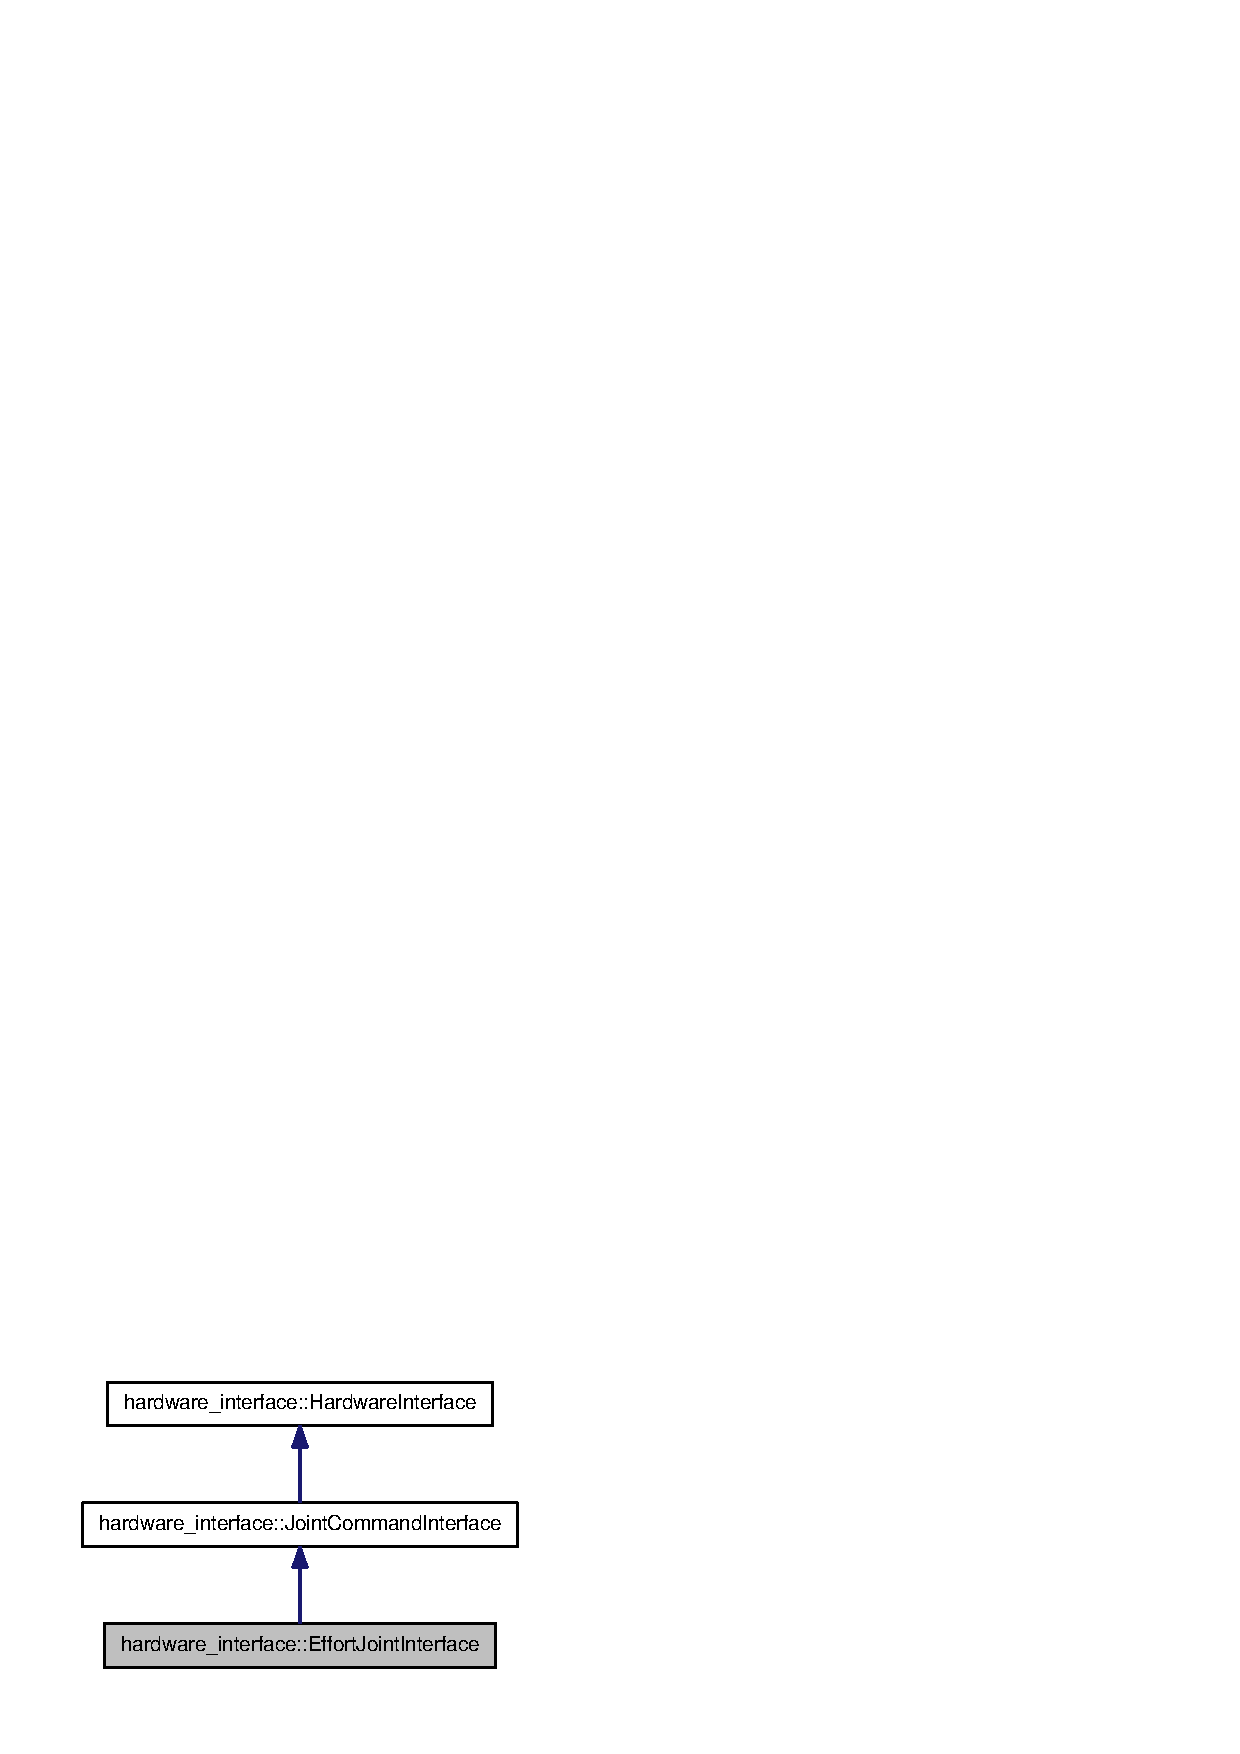
\includegraphics[width=252pt]{classhardware__interface_1_1EffortJointInterface__inherit__graph}
\end{center}
\end{figure}


\subsection{\-Detailed \-Description}
\doxyref{\-Joint\-Command\-Interface}{p.}{classhardware__interface_1_1JointCommandInterface} for commanding effort-\/based joints 

\-Definition at line 120 of file joint\-\_\-command\-\_\-interface.\-h.



\-The documentation for this class was generated from the following file\-:\begin{DoxyCompactItemize}
\item 
{\bf joint\-\_\-command\-\_\-interface.\-h}\end{DoxyCompactItemize}

\section{hardware\-\_\-interface\-:\-:\-Hardware\-Interface \-Class \-Reference}
\label{classhardware__interface_1_1HardwareInterface}\index{hardware\-\_\-interface\-::\-Hardware\-Interface@{hardware\-\_\-interface\-::\-Hardware\-Interface}}


\-Abstract \-Hardware \-Interface.  




{\ttfamily \#include $<$hardware\-\_\-interface.\-h$>$}



\-Inheritance diagram for hardware\-\_\-interface\-:\-:\-Hardware\-Interface\-:
\nopagebreak
\begin{figure}[H]
\begin{center}
\leavevmode
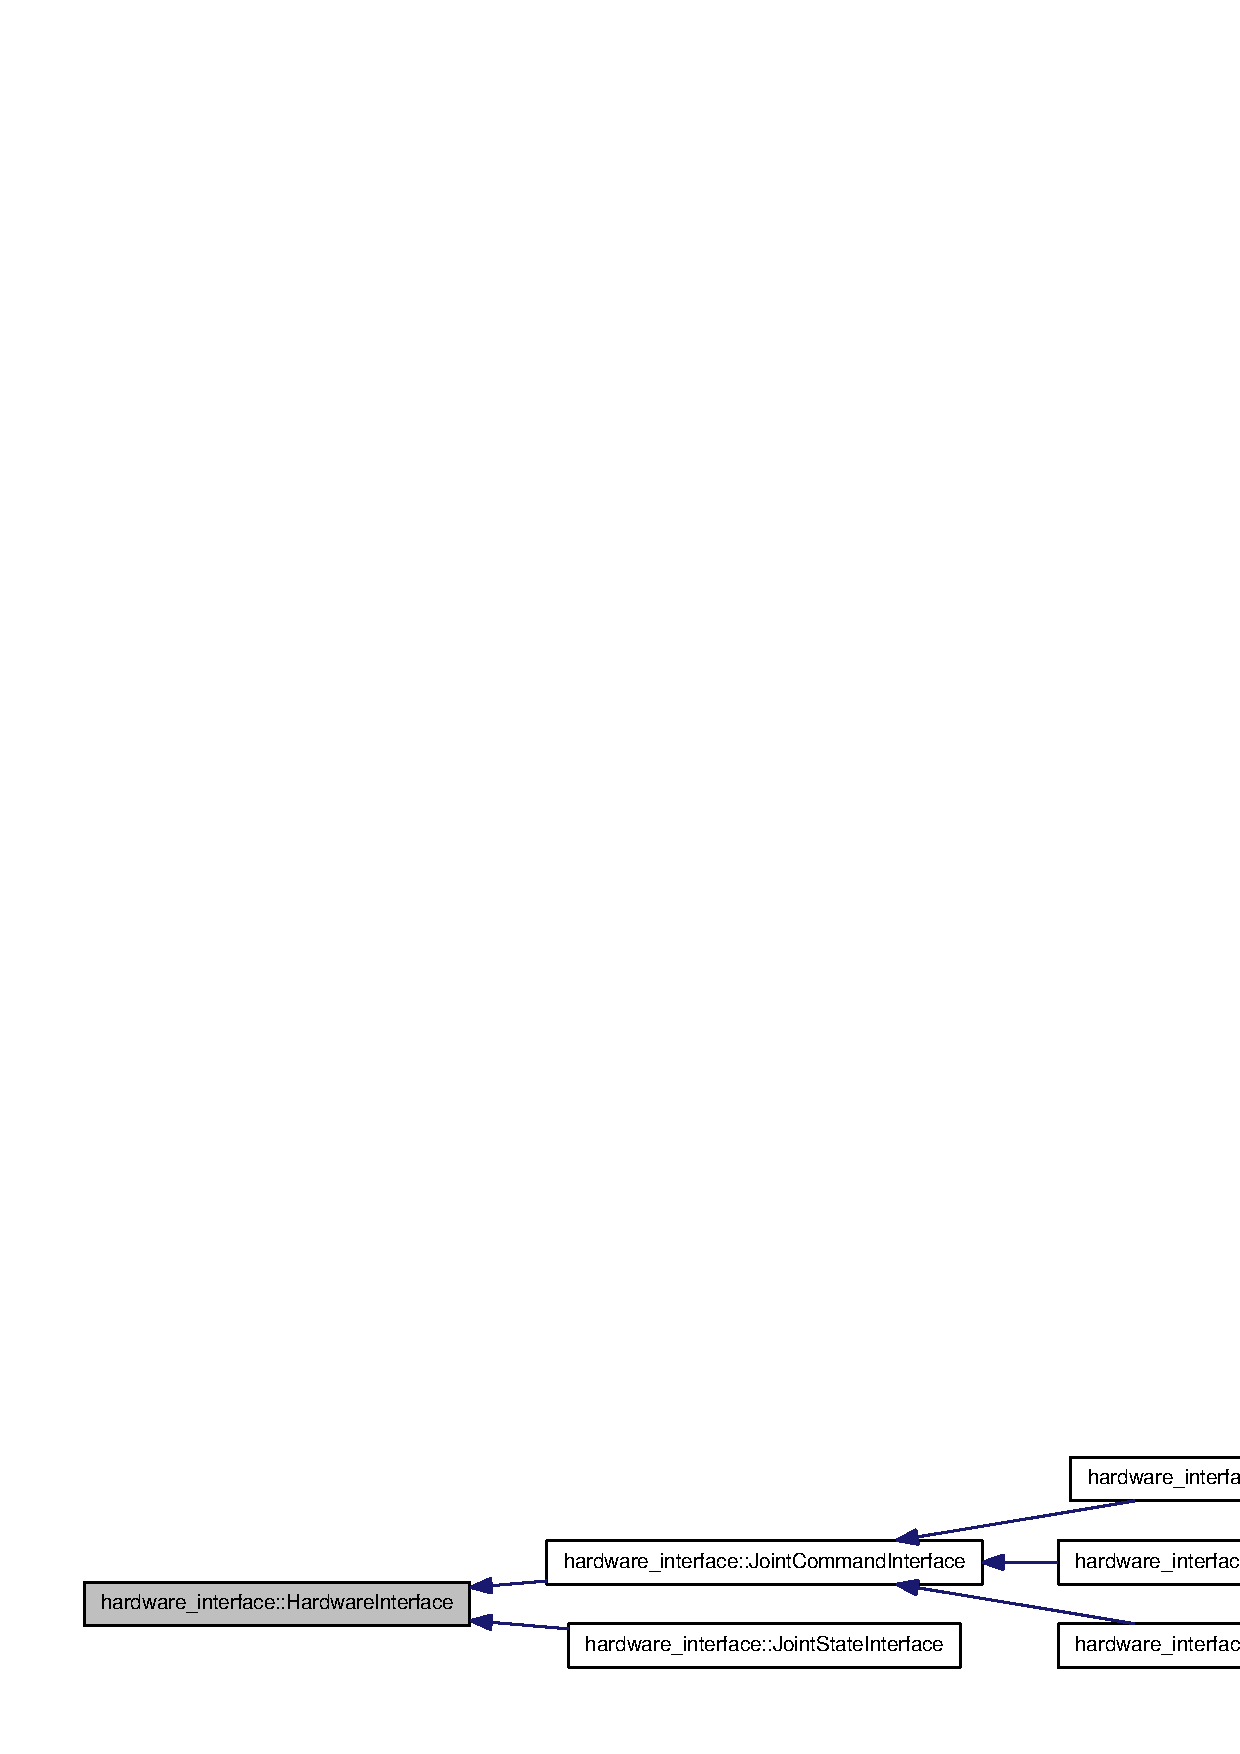
\includegraphics[width=350pt]{classhardware__interface_1_1HardwareInterface__inherit__graph}
\end{center}
\end{figure}
\subsection*{\-Public \-Member \-Functions}
\begin{DoxyCompactItemize}
\item 
virtual {\bf $\sim$\-Hardware\-Interface} ()
\end{DoxyCompactItemize}
\begin{Indent}{\bf \-Resource management}\par
\begin{DoxyCompactItemize}
\item 
virtual void {\bf claim} (std\-::string resource)
\begin{DoxyCompactList}\small\item\em \-Claim a resource by name. \end{DoxyCompactList}\item 
void {\bf clear\-Claims} ()
\begin{DoxyCompactList}\small\item\em \-Clear the resources this interface is claiming. \end{DoxyCompactList}\item 
std\-::set$<$ std\-::string $>$ {\bf get\-Claims} () const 
\begin{DoxyCompactList}\small\item\em \-Get the list of resources this interface is currently claiming. \end{DoxyCompactList}\end{DoxyCompactItemize}
\end{Indent}
\subsection*{\-Private \-Attributes}
\begin{DoxyCompactItemize}
\item 
std\-::set$<$ std\-::string $>$ {\bf claims\-\_\-}
\end{DoxyCompactItemize}


\subsection{\-Detailed \-Description}
\-Abstract \-Hardware \-Interface. 



\-Definition at line 47 of file hardware\-\_\-interface.\-h.



\subsection{\-Constructor \& \-Destructor \-Documentation}
\index{hardware\-\_\-interface\-::\-Hardware\-Interface@{hardware\-\_\-interface\-::\-Hardware\-Interface}!$\sim$\-Hardware\-Interface@{$\sim$\-Hardware\-Interface}}
\index{$\sim$\-Hardware\-Interface@{$\sim$\-Hardware\-Interface}!hardware_interface::HardwareInterface@{hardware\-\_\-interface\-::\-Hardware\-Interface}}
\subsubsection[{$\sim$\-Hardware\-Interface}]{\setlength{\rightskip}{0pt plus 5cm}virtual {\bf hardware\-\_\-interface\-::\-Hardware\-Interface\-::$\sim$\-Hardware\-Interface} (
\begin{DoxyParamCaption}
{}
\end{DoxyParamCaption}
)\hspace{0.3cm}{\ttfamily  [inline, virtual]}}\label{classhardware__interface_1_1HardwareInterface_a66029297e30ce8218aa86db056e73872}


\-Definition at line 50 of file hardware\-\_\-interface.\-h.



\subsection{\-Member \-Function \-Documentation}
\index{hardware\-\_\-interface\-::\-Hardware\-Interface@{hardware\-\_\-interface\-::\-Hardware\-Interface}!claim@{claim}}
\index{claim@{claim}!hardware_interface::HardwareInterface@{hardware\-\_\-interface\-::\-Hardware\-Interface}}
\subsubsection[{claim}]{\setlength{\rightskip}{0pt plus 5cm}virtual void {\bf hardware\-\_\-interface\-::\-Hardware\-Interface\-::claim} (
\begin{DoxyParamCaption}
\item[{std\-::string}]{resource}
\end{DoxyParamCaption}
)\hspace{0.3cm}{\ttfamily  [inline, virtual]}}\label{classhardware__interface_1_1HardwareInterface_a1cbbbf08565bd3b6b602c8150dbf5222}


\-Claim a resource by name. 



\-Definition at line 56 of file hardware\-\_\-interface.\-h.

\index{hardware\-\_\-interface\-::\-Hardware\-Interface@{hardware\-\_\-interface\-::\-Hardware\-Interface}!clear\-Claims@{clear\-Claims}}
\index{clear\-Claims@{clear\-Claims}!hardware_interface::HardwareInterface@{hardware\-\_\-interface\-::\-Hardware\-Interface}}
\subsubsection[{clear\-Claims}]{\setlength{\rightskip}{0pt plus 5cm}void {\bf hardware\-\_\-interface\-::\-Hardware\-Interface\-::clear\-Claims} (
\begin{DoxyParamCaption}
{}
\end{DoxyParamCaption}
)\hspace{0.3cm}{\ttfamily  [inline]}}\label{classhardware__interface_1_1HardwareInterface_ae3dc4c94adb4b1b767d291ce9f97a2ab}


\-Clear the resources this interface is claiming. 



\-Definition at line 59 of file hardware\-\_\-interface.\-h.

\index{hardware\-\_\-interface\-::\-Hardware\-Interface@{hardware\-\_\-interface\-::\-Hardware\-Interface}!get\-Claims@{get\-Claims}}
\index{get\-Claims@{get\-Claims}!hardware_interface::HardwareInterface@{hardware\-\_\-interface\-::\-Hardware\-Interface}}
\subsubsection[{get\-Claims}]{\setlength{\rightskip}{0pt plus 5cm}std\-::set$<$std\-::string$>$ {\bf hardware\-\_\-interface\-::\-Hardware\-Interface\-::get\-Claims} (
\begin{DoxyParamCaption}
{}
\end{DoxyParamCaption}
) const\hspace{0.3cm}{\ttfamily  [inline]}}\label{classhardware__interface_1_1HardwareInterface_aaa6cbe2de90c06134a152059175f5a2e}


\-Get the list of resources this interface is currently claiming. 



\-Definition at line 62 of file hardware\-\_\-interface.\-h.



\subsection{\-Member \-Data \-Documentation}
\index{hardware\-\_\-interface\-::\-Hardware\-Interface@{hardware\-\_\-interface\-::\-Hardware\-Interface}!claims\-\_\-@{claims\-\_\-}}
\index{claims\-\_\-@{claims\-\_\-}!hardware_interface::HardwareInterface@{hardware\-\_\-interface\-::\-Hardware\-Interface}}
\subsubsection[{claims\-\_\-}]{\setlength{\rightskip}{0pt plus 5cm}std\-::set$<$std\-::string$>$ {\bf hardware\-\_\-interface\-::\-Hardware\-Interface\-::claims\-\_\-}\hspace{0.3cm}{\ttfamily  [private]}}\label{classhardware__interface_1_1HardwareInterface_a739621a61c83be71e29200f55fede47d}


\-Definition at line 67 of file hardware\-\_\-interface.\-h.



\-The documentation for this class was generated from the following file\-:\begin{DoxyCompactItemize}
\item 
{\bf hardware\-\_\-interface.\-h}\end{DoxyCompactItemize}

\section{hardware\-\_\-interface\-:\-:\-Hardware\-Interface\-Exception \-Class \-Reference}
\label{classhardware__interface_1_1HardwareInterfaceException}\index{hardware\-\_\-interface\-::\-Hardware\-Interface\-Exception@{hardware\-\_\-interface\-::\-Hardware\-Interface\-Exception}}


\-An exception related to a \doxyref{\-Hardware\-Interface}{p.}{classhardware__interface_1_1HardwareInterface}.  




{\ttfamily \#include $<$hardware\-\_\-interface.\-h$>$}

\subsection*{\-Public \-Member \-Functions}
\begin{DoxyCompactItemize}
\item 
{\bf \-Hardware\-Interface\-Exception} (const std\-::string \&message)
\item 
virtual const char $\ast$ {\bf what} () const   throw ()
\item 
virtual {\bf $\sim$\-Hardware\-Interface\-Exception} ()  throw ()
\end{DoxyCompactItemize}
\subsection*{\-Private \-Attributes}
\begin{DoxyCompactItemize}
\item 
std\-::string {\bf msg}
\end{DoxyCompactItemize}


\subsection{\-Detailed \-Description}
\-An exception related to a \doxyref{\-Hardware\-Interface}{p.}{classhardware__interface_1_1HardwareInterface}. 

\-Definition at line 72 of file hardware\-\_\-interface.\-h.



\subsection{\-Constructor \& \-Destructor \-Documentation}
\index{hardware\-\_\-interface\-::\-Hardware\-Interface\-Exception@{hardware\-\_\-interface\-::\-Hardware\-Interface\-Exception}!\-Hardware\-Interface\-Exception@{\-Hardware\-Interface\-Exception}}
\index{\-Hardware\-Interface\-Exception@{\-Hardware\-Interface\-Exception}!hardware_interface::HardwareInterfaceException@{hardware\-\_\-interface\-::\-Hardware\-Interface\-Exception}}
\subsubsection[{\-Hardware\-Interface\-Exception}]{\setlength{\rightskip}{0pt plus 5cm}{\bf hardware\-\_\-interface\-::\-Hardware\-Interface\-Exception\-::\-Hardware\-Interface\-Exception} (
\begin{DoxyParamCaption}
\item[{const std\-::string \&}]{message}
\end{DoxyParamCaption}
)\hspace{0.3cm}{\ttfamily  [inline]}}\label{classhardware__interface_1_1HardwareInterfaceException_ade3a75f1638b8f011fb9ff2e7492713f}


\-Definition at line 75 of file hardware\-\_\-interface.\-h.

\index{hardware\-\_\-interface\-::\-Hardware\-Interface\-Exception@{hardware\-\_\-interface\-::\-Hardware\-Interface\-Exception}!$\sim$\-Hardware\-Interface\-Exception@{$\sim$\-Hardware\-Interface\-Exception}}
\index{$\sim$\-Hardware\-Interface\-Exception@{$\sim$\-Hardware\-Interface\-Exception}!hardware_interface::HardwareInterfaceException@{hardware\-\_\-interface\-::\-Hardware\-Interface\-Exception}}
\subsubsection[{$\sim$\-Hardware\-Interface\-Exception}]{\setlength{\rightskip}{0pt plus 5cm}virtual {\bf hardware\-\_\-interface\-::\-Hardware\-Interface\-Exception\-::$\sim$\-Hardware\-Interface\-Exception} (
\begin{DoxyParamCaption}
{}
\end{DoxyParamCaption}
)  throw ()\hspace{0.3cm}{\ttfamily  [inline, virtual]}}\label{classhardware__interface_1_1HardwareInterfaceException_acbf6b0d8ed4bdc9f99b91d0d8f362ac8}


\-Definition at line 78 of file hardware\-\_\-interface.\-h.



\subsection{\-Member \-Function \-Documentation}
\index{hardware\-\_\-interface\-::\-Hardware\-Interface\-Exception@{hardware\-\_\-interface\-::\-Hardware\-Interface\-Exception}!what@{what}}
\index{what@{what}!hardware_interface::HardwareInterfaceException@{hardware\-\_\-interface\-::\-Hardware\-Interface\-Exception}}
\subsubsection[{what}]{\setlength{\rightskip}{0pt plus 5cm}virtual const char$\ast$ {\bf hardware\-\_\-interface\-::\-Hardware\-Interface\-Exception\-::what} (
\begin{DoxyParamCaption}
{}
\end{DoxyParamCaption}
) const  throw ()\hspace{0.3cm}{\ttfamily  [inline, virtual]}}\label{classhardware__interface_1_1HardwareInterfaceException_ae97ac9f695ce1815b8729ea58d0ceecb}


\-Definition at line 80 of file hardware\-\_\-interface.\-h.



\subsection{\-Member \-Data \-Documentation}
\index{hardware\-\_\-interface\-::\-Hardware\-Interface\-Exception@{hardware\-\_\-interface\-::\-Hardware\-Interface\-Exception}!msg@{msg}}
\index{msg@{msg}!hardware_interface::HardwareInterfaceException@{hardware\-\_\-interface\-::\-Hardware\-Interface\-Exception}}
\subsubsection[{msg}]{\setlength{\rightskip}{0pt plus 5cm}std\-::string {\bf hardware\-\_\-interface\-::\-Hardware\-Interface\-Exception\-::msg}\hspace{0.3cm}{\ttfamily  [private]}}\label{classhardware__interface_1_1HardwareInterfaceException_ac2798ea2b9faa54dccec1d1d364c224f}


\-Definition at line 87 of file hardware\-\_\-interface.\-h.



\-The documentation for this class was generated from the following file\-:\begin{DoxyCompactItemize}
\item 
{\bf hardware\-\_\-interface.\-h}\end{DoxyCompactItemize}

\section{hardware\-\_\-interface\-:\-:\-Joint\-Command\-Interface \-Class \-Reference}
\label{classhardware__interface_1_1JointCommandInterface}\index{hardware\-\_\-interface\-::\-Joint\-Command\-Interface@{hardware\-\_\-interface\-::\-Joint\-Command\-Interface}}


\-Hardware interface to support commanding an array of joints.  




{\ttfamily \#include $<$joint\-\_\-command\-\_\-interface.\-h$>$}



\-Inheritance diagram for hardware\-\_\-interface\-:\-:\-Joint\-Command\-Interface\-:
\nopagebreak
\begin{figure}[H]
\begin{center}
\leavevmode
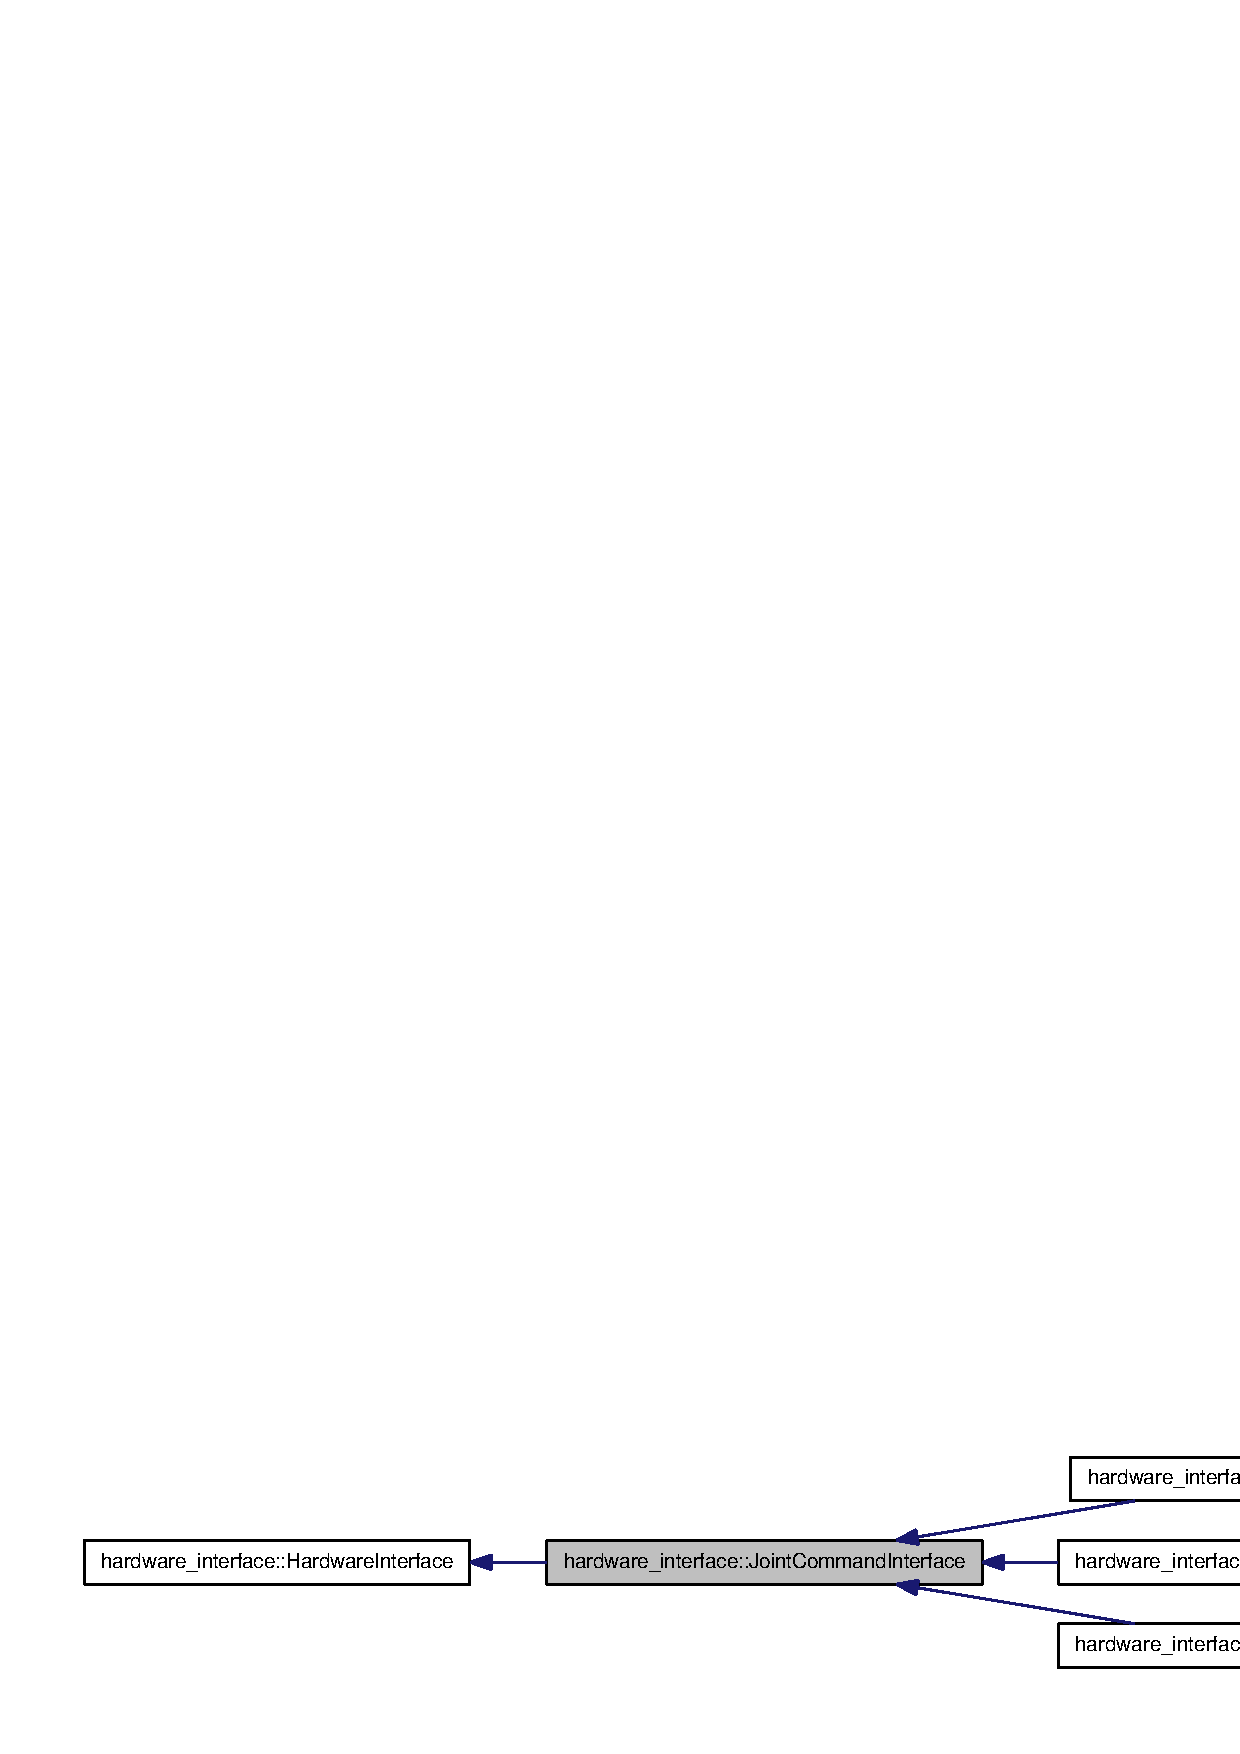
\includegraphics[width=350pt]{classhardware__interface_1_1JointCommandInterface__inherit__graph}
\end{center}
\end{figure}
\subsection*{\-Public \-Member \-Functions}
\begin{DoxyCompactItemize}
\item 
{\bf \-Joint\-Handle} {\bf get\-Joint\-Handle} (const std\-::string \&name)
\begin{DoxyCompactList}\small\item\em \-Get a \doxyref{\-Joint\-Handle}{p.}{classhardware__interface_1_1JointHandle} for accessing a joint's state and setting its output command. \end{DoxyCompactList}\item 
std\-::vector$<$ std\-::string $>$ {\bf get\-Joint\-Names} () const 
\begin{DoxyCompactList}\small\item\em \-Get the vector of joint names registered to this interface. \end{DoxyCompactList}\item 
void {\bf register\-Joint} (const {\bf \-Joint\-State\-Handle} \&js, double $\ast$cmd)
\begin{DoxyCompactList}\small\item\em \-Register a new joint with this interface. \end{DoxyCompactList}\end{DoxyCompactItemize}
\subsection*{\-Protected \-Types}
\begin{DoxyCompactItemize}
\item 
typedef std\-::map$<$ std\-::string, \*
{\bf \-Joint\-Handle} $>$ {\bf \-Handle\-Map}
\end{DoxyCompactItemize}
\subsection*{\-Protected \-Attributes}
\begin{DoxyCompactItemize}
\item 
{\bf \-Handle\-Map} {\bf handle\-\_\-map\-\_\-}
\end{DoxyCompactItemize}


\subsection{\-Detailed \-Description}
\-Hardware interface to support commanding an array of joints. 

\-This \doxyref{\-Hardware\-Interface}{p.}{classhardware__interface_1_1HardwareInterface} supports commanding the output of an array of named joints. \-Note that these commands can have any semantic meaning as long as they each can be represented by a single double, they are not necessarily effort commands. \-To specify a meaning to this command, see the derived classes like \doxyref{\-Effort\-Joint\-Interface}{p.}{classhardware__interface_1_1EffortJointInterface} etc. 

\-Definition at line 62 of file joint\-\_\-command\-\_\-interface.\-h.



\subsection{\-Member \-Typedef \-Documentation}
\index{hardware\-\_\-interface\-::\-Joint\-Command\-Interface@{hardware\-\_\-interface\-::\-Joint\-Command\-Interface}!\-Handle\-Map@{\-Handle\-Map}}
\index{\-Handle\-Map@{\-Handle\-Map}!hardware_interface::JointCommandInterface@{hardware\-\_\-interface\-::\-Joint\-Command\-Interface}}
\subsubsection[{\-Handle\-Map}]{\setlength{\rightskip}{0pt plus 5cm}typedef std\-::map$<$std\-::string, {\bf \-Joint\-Handle}$>$ {\bf hardware\-\_\-interface\-::\-Joint\-Command\-Interface\-::\-Handle\-Map}\hspace{0.3cm}{\ttfamily  [protected]}}\label{classhardware__interface_1_1JointCommandInterface_aedf0d8a77b297ed5b9cb0bf0c2b3e986}


\-Definition at line 115 of file joint\-\_\-command\-\_\-interface.\-h.



\subsection{\-Member \-Function \-Documentation}
\index{hardware\-\_\-interface\-::\-Joint\-Command\-Interface@{hardware\-\_\-interface\-::\-Joint\-Command\-Interface}!get\-Joint\-Handle@{get\-Joint\-Handle}}
\index{get\-Joint\-Handle@{get\-Joint\-Handle}!hardware_interface::JointCommandInterface@{hardware\-\_\-interface\-::\-Joint\-Command\-Interface}}
\subsubsection[{get\-Joint\-Handle}]{\setlength{\rightskip}{0pt plus 5cm}{\bf \-Joint\-Handle} {\bf hardware\-\_\-interface\-::\-Joint\-Command\-Interface\-::get\-Joint\-Handle} (
\begin{DoxyParamCaption}
\item[{const std\-::string \&}]{name}
\end{DoxyParamCaption}
)\hspace{0.3cm}{\ttfamily  [inline]}}\label{classhardware__interface_1_1JointCommandInterface_a07cb2be92559938fdf166f2032dde547}


\-Get a \doxyref{\-Joint\-Handle}{p.}{classhardware__interface_1_1JointHandle} for accessing a joint's state and setting its output command. 

\-When a \doxyref{\-Joint\-Handle}{p.}{classhardware__interface_1_1JointHandle} is acquired, this interface will claim the joint as a resource.


\begin{DoxyParams}{\-Parameters}
{\em name} & \-The name of the joint\\
\hline
\end{DoxyParams}
\begin{DoxyReturn}{\-Returns}
\-A \doxyref{\-Joint\-Handle}{p.}{classhardware__interface_1_1JointHandle} corresponding to the joint identified by {\ttfamily name} 
\end{DoxyReturn}


\-Definition at line 103 of file joint\-\_\-command\-\_\-interface.\-h.

\index{hardware\-\_\-interface\-::\-Joint\-Command\-Interface@{hardware\-\_\-interface\-::\-Joint\-Command\-Interface}!get\-Joint\-Names@{get\-Joint\-Names}}
\index{get\-Joint\-Names@{get\-Joint\-Names}!hardware_interface::JointCommandInterface@{hardware\-\_\-interface\-::\-Joint\-Command\-Interface}}
\subsubsection[{get\-Joint\-Names}]{\setlength{\rightskip}{0pt plus 5cm}std\-::vector$<$std\-::string$>$ {\bf hardware\-\_\-interface\-::\-Joint\-Command\-Interface\-::get\-Joint\-Names} (
\begin{DoxyParamCaption}
{}
\end{DoxyParamCaption}
) const\hspace{0.3cm}{\ttfamily  [inline]}}\label{classhardware__interface_1_1JointCommandInterface_a61861b11cb5d39d09c0c073c24112396}


\-Get the vector of joint names registered to this interface. 



\-Definition at line 66 of file joint\-\_\-command\-\_\-interface.\-h.

\index{hardware\-\_\-interface\-::\-Joint\-Command\-Interface@{hardware\-\_\-interface\-::\-Joint\-Command\-Interface}!register\-Joint@{register\-Joint}}
\index{register\-Joint@{register\-Joint}!hardware_interface::JointCommandInterface@{hardware\-\_\-interface\-::\-Joint\-Command\-Interface}}
\subsubsection[{register\-Joint}]{\setlength{\rightskip}{0pt plus 5cm}void {\bf hardware\-\_\-interface\-::\-Joint\-Command\-Interface\-::register\-Joint} (
\begin{DoxyParamCaption}
\item[{const {\bf \-Joint\-State\-Handle} \&}]{js, }
\item[{double $\ast$}]{cmd}
\end{DoxyParamCaption}
)\hspace{0.3cm}{\ttfamily  [inline]}}\label{classhardware__interface_1_1JointCommandInterface_a423ae65f94c2d21ac647b9a84f4c5fa4}


\-Register a new joint with this interface. 


\begin{DoxyParams}{\-Parameters}
{\em name} & \-The name of the new joint \\
\hline
{\em cmd} & \-A pointer to the storage for this joint's output command \\
\hline
\end{DoxyParams}


\-Definition at line 82 of file joint\-\_\-command\-\_\-interface.\-h.



\subsection{\-Member \-Data \-Documentation}
\index{hardware\-\_\-interface\-::\-Joint\-Command\-Interface@{hardware\-\_\-interface\-::\-Joint\-Command\-Interface}!handle\-\_\-map\-\_\-@{handle\-\_\-map\-\_\-}}
\index{handle\-\_\-map\-\_\-@{handle\-\_\-map\-\_\-}!hardware_interface::JointCommandInterface@{hardware\-\_\-interface\-::\-Joint\-Command\-Interface}}
\subsubsection[{handle\-\_\-map\-\_\-}]{\setlength{\rightskip}{0pt plus 5cm}{\bf \-Handle\-Map} {\bf hardware\-\_\-interface\-::\-Joint\-Command\-Interface\-::handle\-\_\-map\-\_\-}\hspace{0.3cm}{\ttfamily  [protected]}}\label{classhardware__interface_1_1JointCommandInterface_a81b8c65ce8be154d248aee27600aae48}


\-Definition at line 116 of file joint\-\_\-command\-\_\-interface.\-h.



\-The documentation for this class was generated from the following file\-:\begin{DoxyCompactItemize}
\item 
{\bf joint\-\_\-command\-\_\-interface.\-h}\end{DoxyCompactItemize}

\section{hardware\-\_\-interface\-:\-:\-Joint\-Handle \-Class \-Reference}
\label{classhardware__interface_1_1JointHandle}\index{hardware\-\_\-interface\-::\-Joint\-Handle@{hardware\-\_\-interface\-::\-Joint\-Handle}}


\-A handle used to read and command a single joint.  




{\ttfamily \#include $<$joint\-\_\-command\-\_\-interface.\-h$>$}



\-Inheritance diagram for hardware\-\_\-interface\-:\-:\-Joint\-Handle\-:
\nopagebreak
\begin{figure}[H]
\begin{center}
\leavevmode
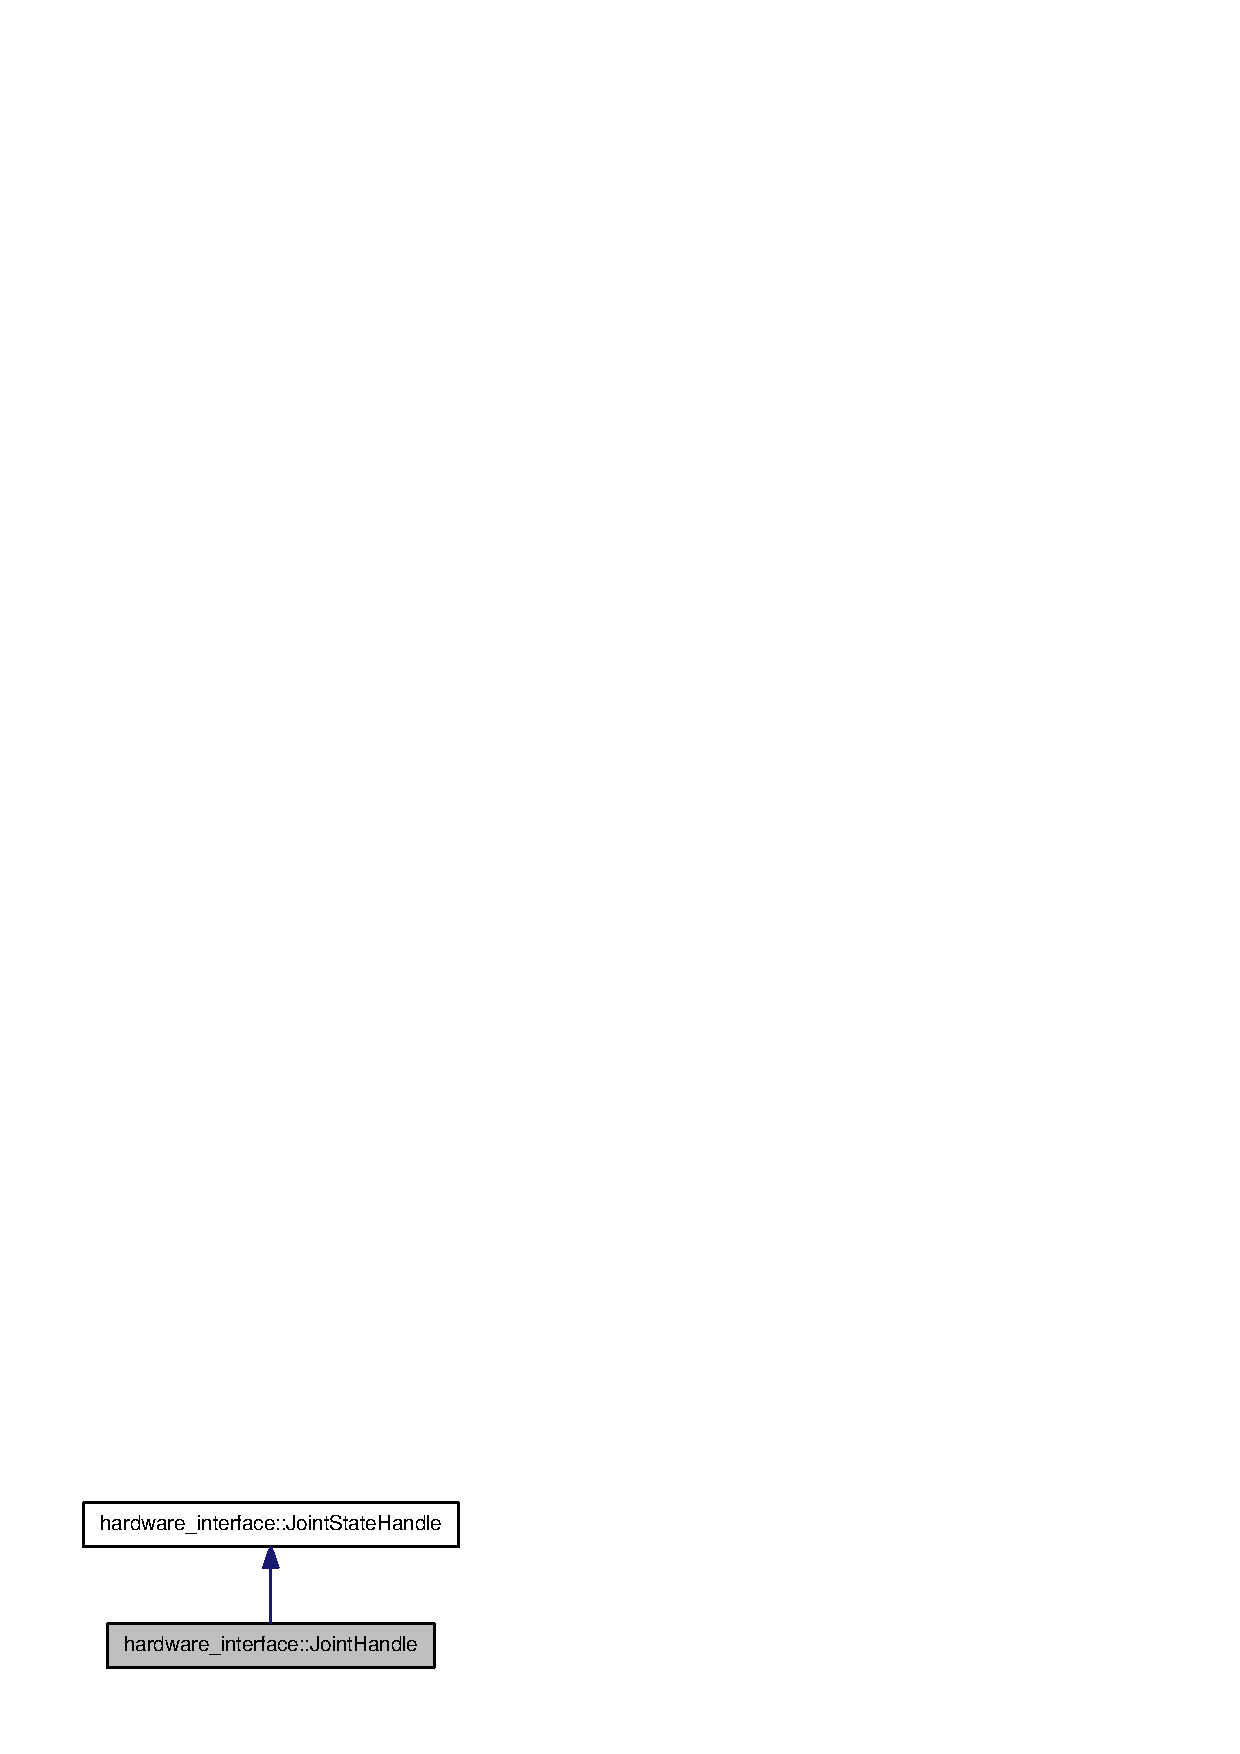
\includegraphics[width=224pt]{classhardware__interface_1_1JointHandle__inherit__graph}
\end{center}
\end{figure}
\subsection*{\-Public \-Member \-Functions}
\begin{DoxyCompactItemize}
\item 
{\bf \-Joint\-Handle} ()
\item 
{\bf \-Joint\-Handle} (const {\bf \-Joint\-State\-Handle} \&js, double $\ast$cmd)
\item 
void {\bf set\-Command} (double command)
\end{DoxyCompactItemize}
\subsection*{\-Private \-Attributes}
\begin{DoxyCompactItemize}
\item 
double $\ast$ {\bf cmd\-\_\-}
\end{DoxyCompactItemize}


\subsection{\-Detailed \-Description}
\-A handle used to read and command a single joint. 

\-Definition at line 39 of file joint\-\_\-command\-\_\-interface.\-h.



\subsection{\-Constructor \& \-Destructor \-Documentation}
\index{hardware\-\_\-interface\-::\-Joint\-Handle@{hardware\-\_\-interface\-::\-Joint\-Handle}!\-Joint\-Handle@{\-Joint\-Handle}}
\index{\-Joint\-Handle@{\-Joint\-Handle}!hardware_interface::JointHandle@{hardware\-\_\-interface\-::\-Joint\-Handle}}
\subsubsection[{\-Joint\-Handle}]{\setlength{\rightskip}{0pt plus 5cm}{\bf hardware\-\_\-interface\-::\-Joint\-Handle\-::\-Joint\-Handle} (
\begin{DoxyParamCaption}
{}
\end{DoxyParamCaption}
)\hspace{0.3cm}{\ttfamily  [inline]}}\label{classhardware__interface_1_1JointHandle_a4aecc1f6251d30cc754ad88168c340ca}


\-Definition at line 42 of file joint\-\_\-command\-\_\-interface.\-h.

\index{hardware\-\_\-interface\-::\-Joint\-Handle@{hardware\-\_\-interface\-::\-Joint\-Handle}!\-Joint\-Handle@{\-Joint\-Handle}}
\index{\-Joint\-Handle@{\-Joint\-Handle}!hardware_interface::JointHandle@{hardware\-\_\-interface\-::\-Joint\-Handle}}
\subsubsection[{\-Joint\-Handle}]{\setlength{\rightskip}{0pt plus 5cm}{\bf hardware\-\_\-interface\-::\-Joint\-Handle\-::\-Joint\-Handle} (
\begin{DoxyParamCaption}
\item[{const {\bf \-Joint\-State\-Handle} \&}]{js, }
\item[{double $\ast$}]{cmd}
\end{DoxyParamCaption}
)\hspace{0.3cm}{\ttfamily  [inline]}}\label{classhardware__interface_1_1JointHandle_a1eae3b1b8498b2f30d73c0c74c1ca0d3}


\-Definition at line 43 of file joint\-\_\-command\-\_\-interface.\-h.



\subsection{\-Member \-Function \-Documentation}
\index{hardware\-\_\-interface\-::\-Joint\-Handle@{hardware\-\_\-interface\-::\-Joint\-Handle}!set\-Command@{set\-Command}}
\index{set\-Command@{set\-Command}!hardware_interface::JointHandle@{hardware\-\_\-interface\-::\-Joint\-Handle}}
\subsubsection[{set\-Command}]{\setlength{\rightskip}{0pt plus 5cm}void {\bf hardware\-\_\-interface\-::\-Joint\-Handle\-::set\-Command} (
\begin{DoxyParamCaption}
\item[{double}]{command}
\end{DoxyParamCaption}
)\hspace{0.3cm}{\ttfamily  [inline]}}\label{classhardware__interface_1_1JointHandle_a352fb0bfb003299f5da75963a1dfbfd6}


\-Definition at line 46 of file joint\-\_\-command\-\_\-interface.\-h.



\subsection{\-Member \-Data \-Documentation}
\index{hardware\-\_\-interface\-::\-Joint\-Handle@{hardware\-\_\-interface\-::\-Joint\-Handle}!cmd\-\_\-@{cmd\-\_\-}}
\index{cmd\-\_\-@{cmd\-\_\-}!hardware_interface::JointHandle@{hardware\-\_\-interface\-::\-Joint\-Handle}}
\subsubsection[{cmd\-\_\-}]{\setlength{\rightskip}{0pt plus 5cm}double$\ast$ {\bf hardware\-\_\-interface\-::\-Joint\-Handle\-::cmd\-\_\-}\hspace{0.3cm}{\ttfamily  [private]}}\label{classhardware__interface_1_1JointHandle_a8ca98df67c80ec5dfa76ced341c73abf}


\-Definition at line 46 of file joint\-\_\-command\-\_\-interface.\-h.



\-The documentation for this class was generated from the following file\-:\begin{DoxyCompactItemize}
\item 
{\bf joint\-\_\-command\-\_\-interface.\-h}\end{DoxyCompactItemize}

\section{hardware\-\_\-interface\-:\-:\-Joint\-State\-Handle \-Class \-Reference}
\label{classhardware__interface_1_1JointStateHandle}\index{hardware\-\_\-interface\-::\-Joint\-State\-Handle@{hardware\-\_\-interface\-::\-Joint\-State\-Handle}}


\-A handle used to read the state of a single joint.  




{\ttfamily \#include $<$joint\-\_\-state\-\_\-interface.\-h$>$}



\-Inheritance diagram for hardware\-\_\-interface\-:\-:\-Joint\-State\-Handle\-:
\nopagebreak
\begin{figure}[H]
\begin{center}
\leavevmode
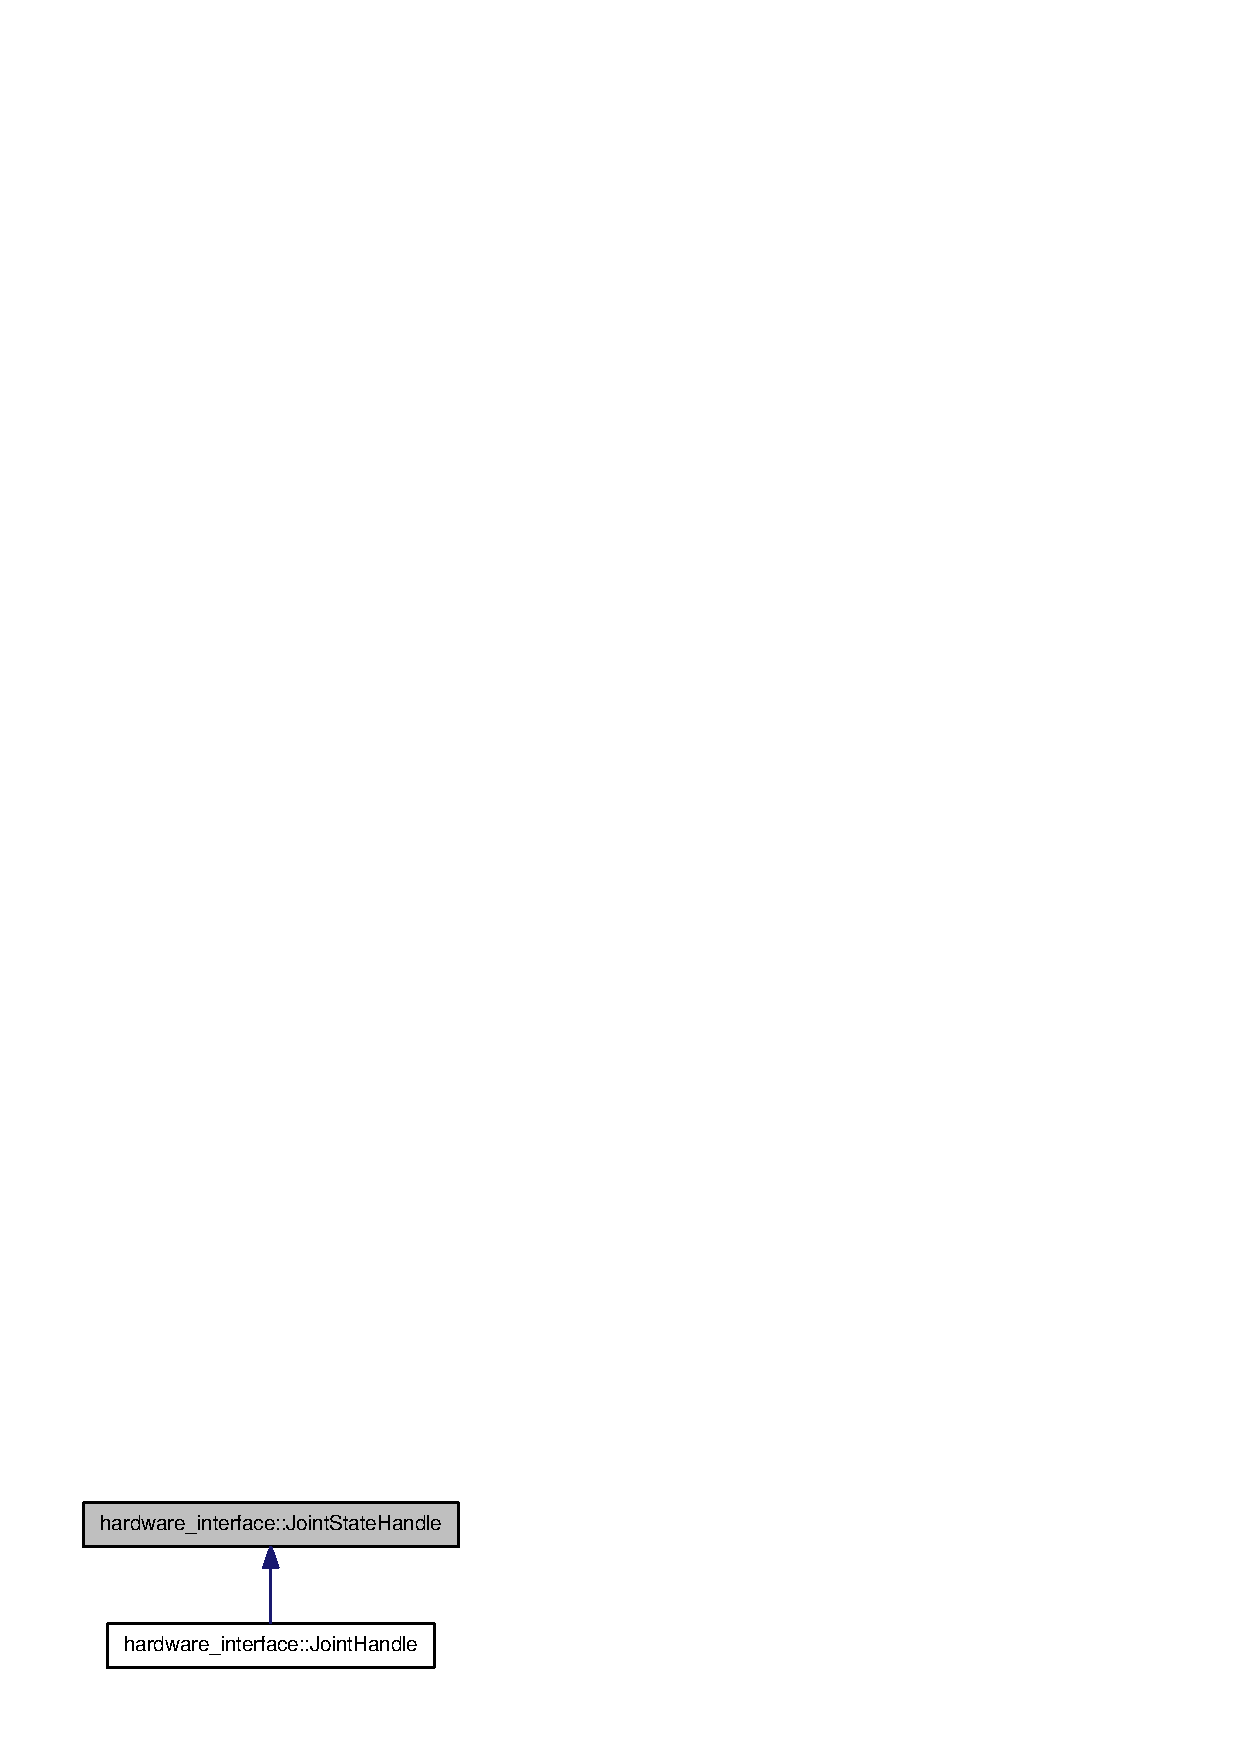
\includegraphics[width=224pt]{classhardware__interface_1_1JointStateHandle__inherit__graph}
\end{center}
\end{figure}
\subsection*{\-Public \-Member \-Functions}
\begin{DoxyCompactItemize}
\item 
double {\bf get\-Effort} () const 
\item 
std\-::string {\bf get\-Name} () const 
\item 
double {\bf get\-Position} () const 
\item 
double {\bf get\-Velocity} () const 
\item 
{\bf \-Joint\-State\-Handle} ()
\item 
{\bf \-Joint\-State\-Handle} (const std\-::string \&name, const double $\ast$pos, const double $\ast$vel, const double $\ast$eff)
\end{DoxyCompactItemize}
\subsection*{\-Private \-Attributes}
\begin{DoxyCompactItemize}
\item 
const double $\ast$ {\bf eff\-\_\-}
\item 
std\-::string {\bf name\-\_\-}
\item 
const double $\ast$ {\bf pos\-\_\-}
\item 
const double $\ast$ {\bf vel\-\_\-}
\end{DoxyCompactItemize}


\subsection{\-Detailed \-Description}
\-A handle used to read the state of a single joint. 

\-Definition at line 44 of file joint\-\_\-state\-\_\-interface.\-h.



\subsection{\-Constructor \& \-Destructor \-Documentation}
\index{hardware\-\_\-interface\-::\-Joint\-State\-Handle@{hardware\-\_\-interface\-::\-Joint\-State\-Handle}!\-Joint\-State\-Handle@{\-Joint\-State\-Handle}}
\index{\-Joint\-State\-Handle@{\-Joint\-State\-Handle}!hardware_interface::JointStateHandle@{hardware\-\_\-interface\-::\-Joint\-State\-Handle}}
\subsubsection[{\-Joint\-State\-Handle}]{\setlength{\rightskip}{0pt plus 5cm}{\bf hardware\-\_\-interface\-::\-Joint\-State\-Handle\-::\-Joint\-State\-Handle} (
\begin{DoxyParamCaption}
{}
\end{DoxyParamCaption}
)\hspace{0.3cm}{\ttfamily  [inline]}}\label{classhardware__interface_1_1JointStateHandle_a7bd20af3c9edd0ce90e21ed7e0dc91f7}


\-Definition at line 47 of file joint\-\_\-state\-\_\-interface.\-h.

\index{hardware\-\_\-interface\-::\-Joint\-State\-Handle@{hardware\-\_\-interface\-::\-Joint\-State\-Handle}!\-Joint\-State\-Handle@{\-Joint\-State\-Handle}}
\index{\-Joint\-State\-Handle@{\-Joint\-State\-Handle}!hardware_interface::JointStateHandle@{hardware\-\_\-interface\-::\-Joint\-State\-Handle}}
\subsubsection[{\-Joint\-State\-Handle}]{\setlength{\rightskip}{0pt plus 5cm}{\bf hardware\-\_\-interface\-::\-Joint\-State\-Handle\-::\-Joint\-State\-Handle} (
\begin{DoxyParamCaption}
\item[{const std\-::string \&}]{name, }
\item[{const double $\ast$}]{pos, }
\item[{const double $\ast$}]{vel, }
\item[{const double $\ast$}]{eff}
\end{DoxyParamCaption}
)\hspace{0.3cm}{\ttfamily  [inline]}}\label{classhardware__interface_1_1JointStateHandle_a329e5e8b72cb2b4c0fd23e28b7b24a2b}


\-Definition at line 48 of file joint\-\_\-state\-\_\-interface.\-h.



\subsection{\-Member \-Function \-Documentation}
\index{hardware\-\_\-interface\-::\-Joint\-State\-Handle@{hardware\-\_\-interface\-::\-Joint\-State\-Handle}!get\-Effort@{get\-Effort}}
\index{get\-Effort@{get\-Effort}!hardware_interface::JointStateHandle@{hardware\-\_\-interface\-::\-Joint\-State\-Handle}}
\subsubsection[{get\-Effort}]{\setlength{\rightskip}{0pt plus 5cm}double {\bf hardware\-\_\-interface\-::\-Joint\-State\-Handle\-::get\-Effort} (
\begin{DoxyParamCaption}
{}
\end{DoxyParamCaption}
) const\hspace{0.3cm}{\ttfamily  [inline]}}\label{classhardware__interface_1_1JointStateHandle_a8639df80b2cf72db487a9275b5714a06}


\-Definition at line 55 of file joint\-\_\-state\-\_\-interface.\-h.

\index{hardware\-\_\-interface\-::\-Joint\-State\-Handle@{hardware\-\_\-interface\-::\-Joint\-State\-Handle}!get\-Name@{get\-Name}}
\index{get\-Name@{get\-Name}!hardware_interface::JointStateHandle@{hardware\-\_\-interface\-::\-Joint\-State\-Handle}}
\subsubsection[{get\-Name}]{\setlength{\rightskip}{0pt plus 5cm}std\-::string {\bf hardware\-\_\-interface\-::\-Joint\-State\-Handle\-::get\-Name} (
\begin{DoxyParamCaption}
{}
\end{DoxyParamCaption}
) const\hspace{0.3cm}{\ttfamily  [inline]}}\label{classhardware__interface_1_1JointStateHandle_a660b5cb37f7831b4fcf96b5c0cded55c}


\-Definition at line 52 of file joint\-\_\-state\-\_\-interface.\-h.

\index{hardware\-\_\-interface\-::\-Joint\-State\-Handle@{hardware\-\_\-interface\-::\-Joint\-State\-Handle}!get\-Position@{get\-Position}}
\index{get\-Position@{get\-Position}!hardware_interface::JointStateHandle@{hardware\-\_\-interface\-::\-Joint\-State\-Handle}}
\subsubsection[{get\-Position}]{\setlength{\rightskip}{0pt plus 5cm}double {\bf hardware\-\_\-interface\-::\-Joint\-State\-Handle\-::get\-Position} (
\begin{DoxyParamCaption}
{}
\end{DoxyParamCaption}
) const\hspace{0.3cm}{\ttfamily  [inline]}}\label{classhardware__interface_1_1JointStateHandle_aa04f165441281b570c31b104378ab8e6}


\-Definition at line 53 of file joint\-\_\-state\-\_\-interface.\-h.

\index{hardware\-\_\-interface\-::\-Joint\-State\-Handle@{hardware\-\_\-interface\-::\-Joint\-State\-Handle}!get\-Velocity@{get\-Velocity}}
\index{get\-Velocity@{get\-Velocity}!hardware_interface::JointStateHandle@{hardware\-\_\-interface\-::\-Joint\-State\-Handle}}
\subsubsection[{get\-Velocity}]{\setlength{\rightskip}{0pt plus 5cm}double {\bf hardware\-\_\-interface\-::\-Joint\-State\-Handle\-::get\-Velocity} (
\begin{DoxyParamCaption}
{}
\end{DoxyParamCaption}
) const\hspace{0.3cm}{\ttfamily  [inline]}}\label{classhardware__interface_1_1JointStateHandle_a7c2cfc140d50fd092d51bd0e825bc4a0}


\-Definition at line 54 of file joint\-\_\-state\-\_\-interface.\-h.



\subsection{\-Member \-Data \-Documentation}
\index{hardware\-\_\-interface\-::\-Joint\-State\-Handle@{hardware\-\_\-interface\-::\-Joint\-State\-Handle}!eff\-\_\-@{eff\-\_\-}}
\index{eff\-\_\-@{eff\-\_\-}!hardware_interface::JointStateHandle@{hardware\-\_\-interface\-::\-Joint\-State\-Handle}}
\subsubsection[{eff\-\_\-}]{\setlength{\rightskip}{0pt plus 5cm}const double$\ast$ {\bf hardware\-\_\-interface\-::\-Joint\-State\-Handle\-::eff\-\_\-}\hspace{0.3cm}{\ttfamily  [private]}}\label{classhardware__interface_1_1JointStateHandle_a0ec1a0c886b7dacc616090bef82f4c80}


\-Definition at line 61 of file joint\-\_\-state\-\_\-interface.\-h.

\index{hardware\-\_\-interface\-::\-Joint\-State\-Handle@{hardware\-\_\-interface\-::\-Joint\-State\-Handle}!name\-\_\-@{name\-\_\-}}
\index{name\-\_\-@{name\-\_\-}!hardware_interface::JointStateHandle@{hardware\-\_\-interface\-::\-Joint\-State\-Handle}}
\subsubsection[{name\-\_\-}]{\setlength{\rightskip}{0pt plus 5cm}std\-::string {\bf hardware\-\_\-interface\-::\-Joint\-State\-Handle\-::name\-\_\-}\hspace{0.3cm}{\ttfamily  [private]}}\label{classhardware__interface_1_1JointStateHandle_a907ee3caeb0ee79275ca1aabe13a3802}


\-Definition at line 58 of file joint\-\_\-state\-\_\-interface.\-h.

\index{hardware\-\_\-interface\-::\-Joint\-State\-Handle@{hardware\-\_\-interface\-::\-Joint\-State\-Handle}!pos\-\_\-@{pos\-\_\-}}
\index{pos\-\_\-@{pos\-\_\-}!hardware_interface::JointStateHandle@{hardware\-\_\-interface\-::\-Joint\-State\-Handle}}
\subsubsection[{pos\-\_\-}]{\setlength{\rightskip}{0pt plus 5cm}const double$\ast$ {\bf hardware\-\_\-interface\-::\-Joint\-State\-Handle\-::pos\-\_\-}\hspace{0.3cm}{\ttfamily  [private]}}\label{classhardware__interface_1_1JointStateHandle_ab8550eb758f049d1a3dcd7c0fb7cc185}


\-Definition at line 59 of file joint\-\_\-state\-\_\-interface.\-h.

\index{hardware\-\_\-interface\-::\-Joint\-State\-Handle@{hardware\-\_\-interface\-::\-Joint\-State\-Handle}!vel\-\_\-@{vel\-\_\-}}
\index{vel\-\_\-@{vel\-\_\-}!hardware_interface::JointStateHandle@{hardware\-\_\-interface\-::\-Joint\-State\-Handle}}
\subsubsection[{vel\-\_\-}]{\setlength{\rightskip}{0pt plus 5cm}const double$\ast$ {\bf hardware\-\_\-interface\-::\-Joint\-State\-Handle\-::vel\-\_\-}\hspace{0.3cm}{\ttfamily  [private]}}\label{classhardware__interface_1_1JointStateHandle_aaa0ac8272dee92ee297cbc49f8553991}


\-Definition at line 60 of file joint\-\_\-state\-\_\-interface.\-h.



\-The documentation for this class was generated from the following file\-:\begin{DoxyCompactItemize}
\item 
{\bf joint\-\_\-state\-\_\-interface.\-h}\end{DoxyCompactItemize}

\section{hardware\-\_\-interface\-:\-:\-Joint\-State\-Interface \-Class \-Reference}
\label{classhardware__interface_1_1JointStateInterface}\index{hardware\-\_\-interface\-::\-Joint\-State\-Interface@{hardware\-\_\-interface\-::\-Joint\-State\-Interface}}


\-Hardware interface to support reading the state of an array of joints.  




{\ttfamily \#include $<$joint\-\_\-state\-\_\-interface.\-h$>$}



\-Inheritance diagram for hardware\-\_\-interface\-:\-:\-Joint\-State\-Interface\-:
\nopagebreak
\begin{figure}[H]
\begin{center}
\leavevmode
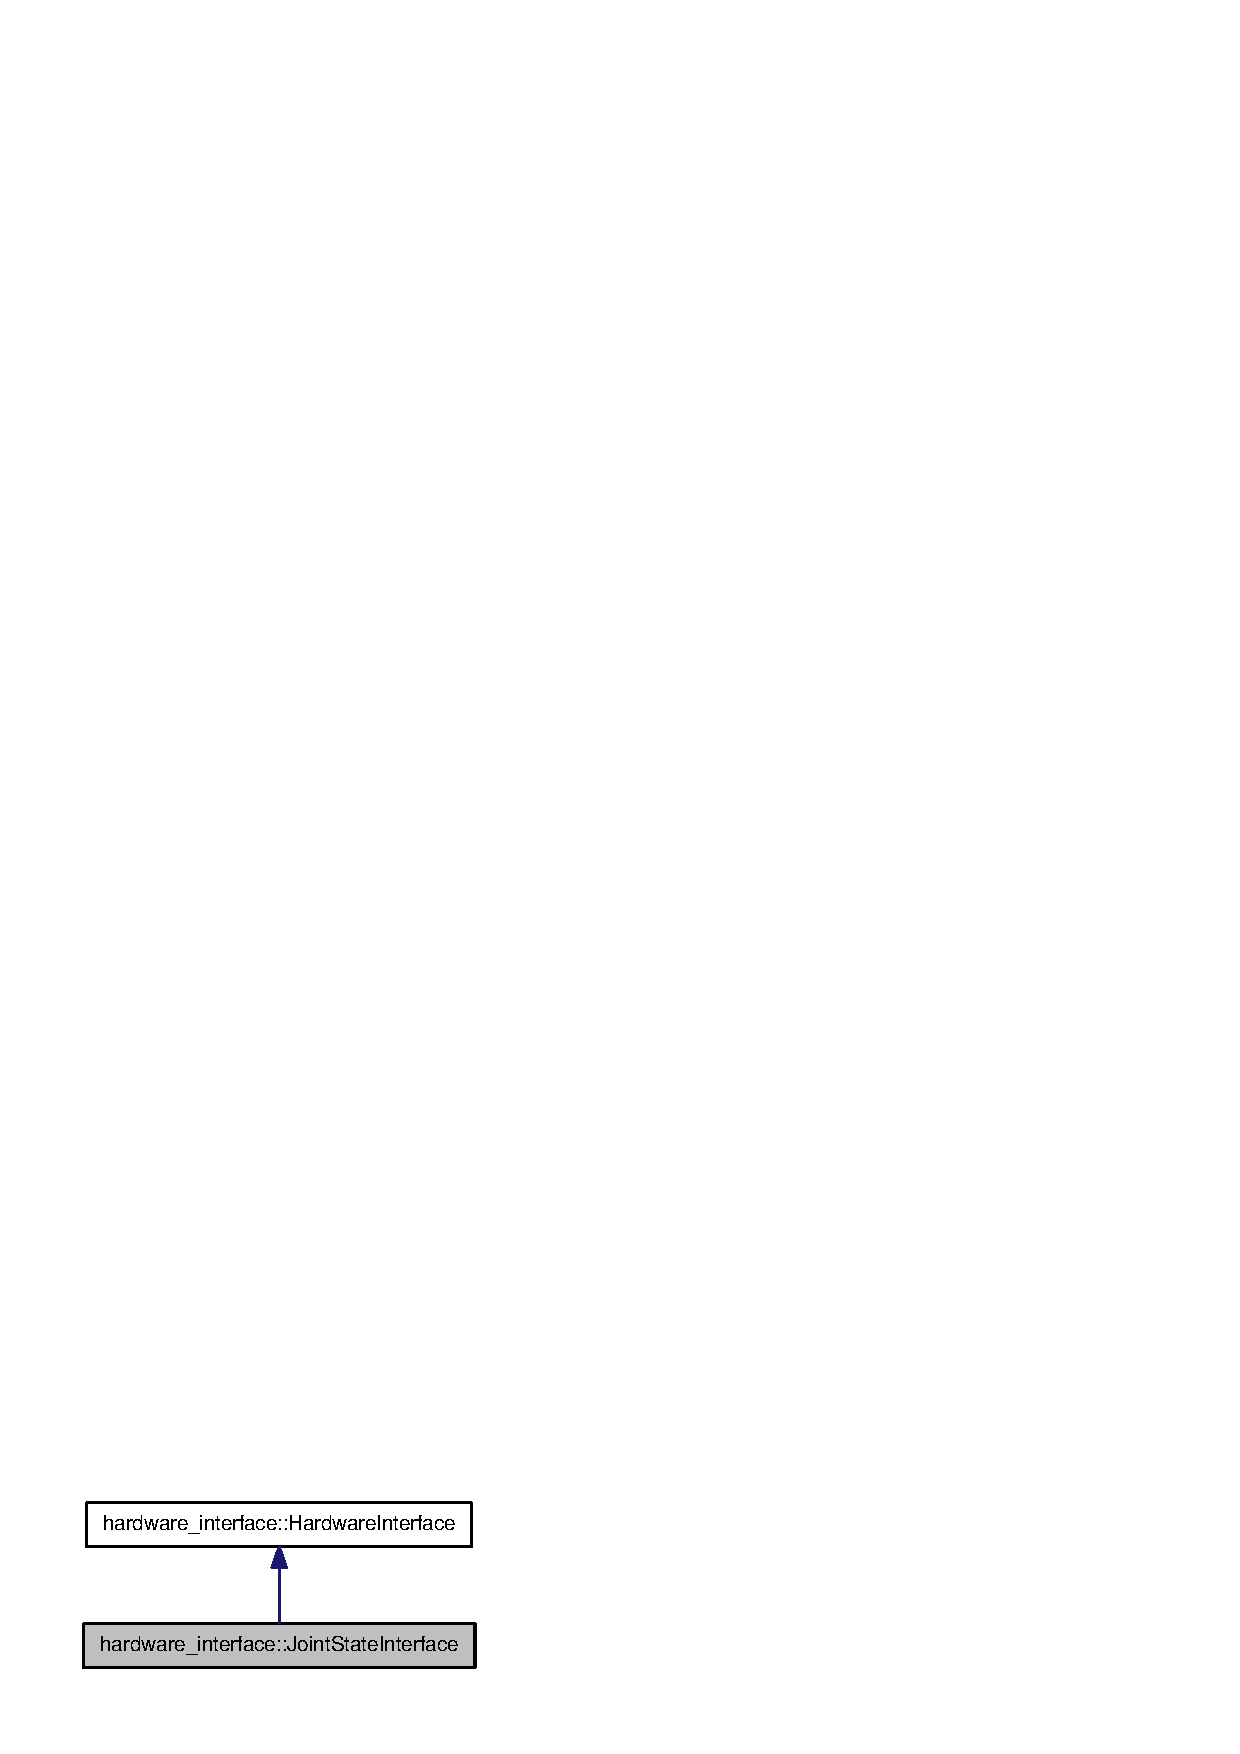
\includegraphics[width=232pt]{classhardware__interface_1_1JointStateInterface__inherit__graph}
\end{center}
\end{figure}
\subsection*{\-Public \-Member \-Functions}
\begin{DoxyCompactItemize}
\item 
std\-::vector$<$ std\-::string $>$ {\bf get\-Joint\-Names} () const 
\begin{DoxyCompactList}\small\item\em \-Get the vector of joint names registered to this interface. \end{DoxyCompactList}\item 
{\bf \-Joint\-State\-Handle} {\bf get\-Joint\-State\-Handle} (const std\-::string \&name) const 
\begin{DoxyCompactList}\small\item\em \-Get a \doxyref{\-Joint\-State\-Handle}{p.}{classhardware__interface_1_1JointStateHandle} for accessing a joint's state. \end{DoxyCompactList}\item 
void {\bf register\-Joint} (const std\-::string \&name, double $\ast$pos, double $\ast$vel, double $\ast$eff)
\begin{DoxyCompactList}\small\item\em \-Register a new joint with this interface. \end{DoxyCompactList}\end{DoxyCompactItemize}
\subsection*{\-Private \-Types}
\begin{DoxyCompactItemize}
\item 
typedef std\-::map$<$ std\-::string, \*
{\bf \-Joint\-State\-Handle} $>$ {\bf \-Handle\-Map}
\end{DoxyCompactItemize}
\subsection*{\-Private \-Attributes}
\begin{DoxyCompactItemize}
\item 
{\bf \-Handle\-Map} {\bf handle\-\_\-map\-\_\-}
\end{DoxyCompactItemize}


\subsection{\-Detailed \-Description}
\-Hardware interface to support reading the state of an array of joints. 

\-This \doxyref{\-Hardware\-Interface}{p.}{classhardware__interface_1_1HardwareInterface} supports reading the state of an array of named joints, each of which has some position, velocity, and effort (force or torque). 

\-Definition at line 72 of file joint\-\_\-state\-\_\-interface.\-h.



\subsection{\-Member \-Typedef \-Documentation}
\index{hardware\-\_\-interface\-::\-Joint\-State\-Interface@{hardware\-\_\-interface\-::\-Joint\-State\-Interface}!\-Handle\-Map@{\-Handle\-Map}}
\index{\-Handle\-Map@{\-Handle\-Map}!hardware_interface::JointStateInterface@{hardware\-\_\-interface\-::\-Joint\-State\-Interface}}
\subsubsection[{\-Handle\-Map}]{\setlength{\rightskip}{0pt plus 5cm}typedef std\-::map$<$std\-::string, {\bf \-Joint\-State\-Handle}$>$ {\bf hardware\-\_\-interface\-::\-Joint\-State\-Interface\-::\-Handle\-Map}\hspace{0.3cm}{\ttfamily  [private]}}\label{classhardware__interface_1_1JointStateInterface_a16048cc6a84711b67f3fc60a2bdf920f}


\-Definition at line 121 of file joint\-\_\-state\-\_\-interface.\-h.



\subsection{\-Member \-Function \-Documentation}
\index{hardware\-\_\-interface\-::\-Joint\-State\-Interface@{hardware\-\_\-interface\-::\-Joint\-State\-Interface}!get\-Joint\-Names@{get\-Joint\-Names}}
\index{get\-Joint\-Names@{get\-Joint\-Names}!hardware_interface::JointStateInterface@{hardware\-\_\-interface\-::\-Joint\-State\-Interface}}
\subsubsection[{get\-Joint\-Names}]{\setlength{\rightskip}{0pt plus 5cm}std\-::vector$<$std\-::string$>$ {\bf hardware\-\_\-interface\-::\-Joint\-State\-Interface\-::get\-Joint\-Names} (
\begin{DoxyParamCaption}
{}
\end{DoxyParamCaption}
) const\hspace{0.3cm}{\ttfamily  [inline]}}\label{classhardware__interface_1_1JointStateInterface_a54b7d366141f8b111a9afa84b6776aa0}


\-Get the vector of joint names registered to this interface. 



\-Definition at line 76 of file joint\-\_\-state\-\_\-interface.\-h.

\index{hardware\-\_\-interface\-::\-Joint\-State\-Interface@{hardware\-\_\-interface\-::\-Joint\-State\-Interface}!get\-Joint\-State\-Handle@{get\-Joint\-State\-Handle}}
\index{get\-Joint\-State\-Handle@{get\-Joint\-State\-Handle}!hardware_interface::JointStateInterface@{hardware\-\_\-interface\-::\-Joint\-State\-Interface}}
\subsubsection[{get\-Joint\-State\-Handle}]{\setlength{\rightskip}{0pt plus 5cm}{\bf \-Joint\-State\-Handle} {\bf hardware\-\_\-interface\-::\-Joint\-State\-Interface\-::get\-Joint\-State\-Handle} (
\begin{DoxyParamCaption}
\item[{const std\-::string \&}]{name}
\end{DoxyParamCaption}
) const\hspace{0.3cm}{\ttfamily  [inline]}}\label{classhardware__interface_1_1JointStateInterface_a734f7ffbb62522ff6201ce053ff471d9}


\-Get a \doxyref{\-Joint\-State\-Handle}{p.}{classhardware__interface_1_1JointStateHandle} for accessing a joint's state. 


\begin{DoxyParams}{\-Parameters}
{\em name} & \-The name of the joint \\
\hline
\end{DoxyParams}


\-Definition at line 110 of file joint\-\_\-state\-\_\-interface.\-h.

\index{hardware\-\_\-interface\-::\-Joint\-State\-Interface@{hardware\-\_\-interface\-::\-Joint\-State\-Interface}!register\-Joint@{register\-Joint}}
\index{register\-Joint@{register\-Joint}!hardware_interface::JointStateInterface@{hardware\-\_\-interface\-::\-Joint\-State\-Interface}}
\subsubsection[{register\-Joint}]{\setlength{\rightskip}{0pt plus 5cm}void {\bf hardware\-\_\-interface\-::\-Joint\-State\-Interface\-::register\-Joint} (
\begin{DoxyParamCaption}
\item[{const std\-::string \&}]{name, }
\item[{double $\ast$}]{pos, }
\item[{double $\ast$}]{vel, }
\item[{double $\ast$}]{eff}
\end{DoxyParamCaption}
)\hspace{0.3cm}{\ttfamily  [inline]}}\label{classhardware__interface_1_1JointStateInterface_a9b81f5830e05013199706d6e5ab98f69}


\-Register a new joint with this interface. 


\begin{DoxyParams}{\-Parameters}
{\em name} & \-The name of the new joint \\
\hline
{\em pos} & \-A pointer to the storage for this joint's position \\
\hline
{\em vel} & \-A pointer to the storage for this joint's velocity \\
\hline
{\em eff} & \-A pointer to the storage for this joint's effort (force or torque) \\
\hline
\end{DoxyParams}


\-Definition at line 95 of file joint\-\_\-state\-\_\-interface.\-h.



\subsection{\-Member \-Data \-Documentation}
\index{hardware\-\_\-interface\-::\-Joint\-State\-Interface@{hardware\-\_\-interface\-::\-Joint\-State\-Interface}!handle\-\_\-map\-\_\-@{handle\-\_\-map\-\_\-}}
\index{handle\-\_\-map\-\_\-@{handle\-\_\-map\-\_\-}!hardware_interface::JointStateInterface@{hardware\-\_\-interface\-::\-Joint\-State\-Interface}}
\subsubsection[{handle\-\_\-map\-\_\-}]{\setlength{\rightskip}{0pt plus 5cm}{\bf \-Handle\-Map} {\bf hardware\-\_\-interface\-::\-Joint\-State\-Interface\-::handle\-\_\-map\-\_\-}\hspace{0.3cm}{\ttfamily  [private]}}\label{classhardware__interface_1_1JointStateInterface_a3e0e78c4b74b1e501c036b498f7aef6e}


\-Definition at line 122 of file joint\-\_\-state\-\_\-interface.\-h.



\-The documentation for this class was generated from the following file\-:\begin{DoxyCompactItemize}
\item 
{\bf joint\-\_\-state\-\_\-interface.\-h}\end{DoxyCompactItemize}

\section{hardware\-\_\-interface\-:\-:\-Position\-Joint\-Interface \-Class \-Reference}
\label{classhardware__interface_1_1PositionJointInterface}\index{hardware\-\_\-interface\-::\-Position\-Joint\-Interface@{hardware\-\_\-interface\-::\-Position\-Joint\-Interface}}


\doxyref{\-Joint\-Command\-Interface}{p.}{classhardware__interface_1_1JointCommandInterface} for commanding position-\/based joints  




{\ttfamily \#include $<$joint\-\_\-command\-\_\-interface.\-h$>$}



\-Inheritance diagram for hardware\-\_\-interface\-:\-:\-Position\-Joint\-Interface\-:
\nopagebreak
\begin{figure}[H]
\begin{center}
\leavevmode
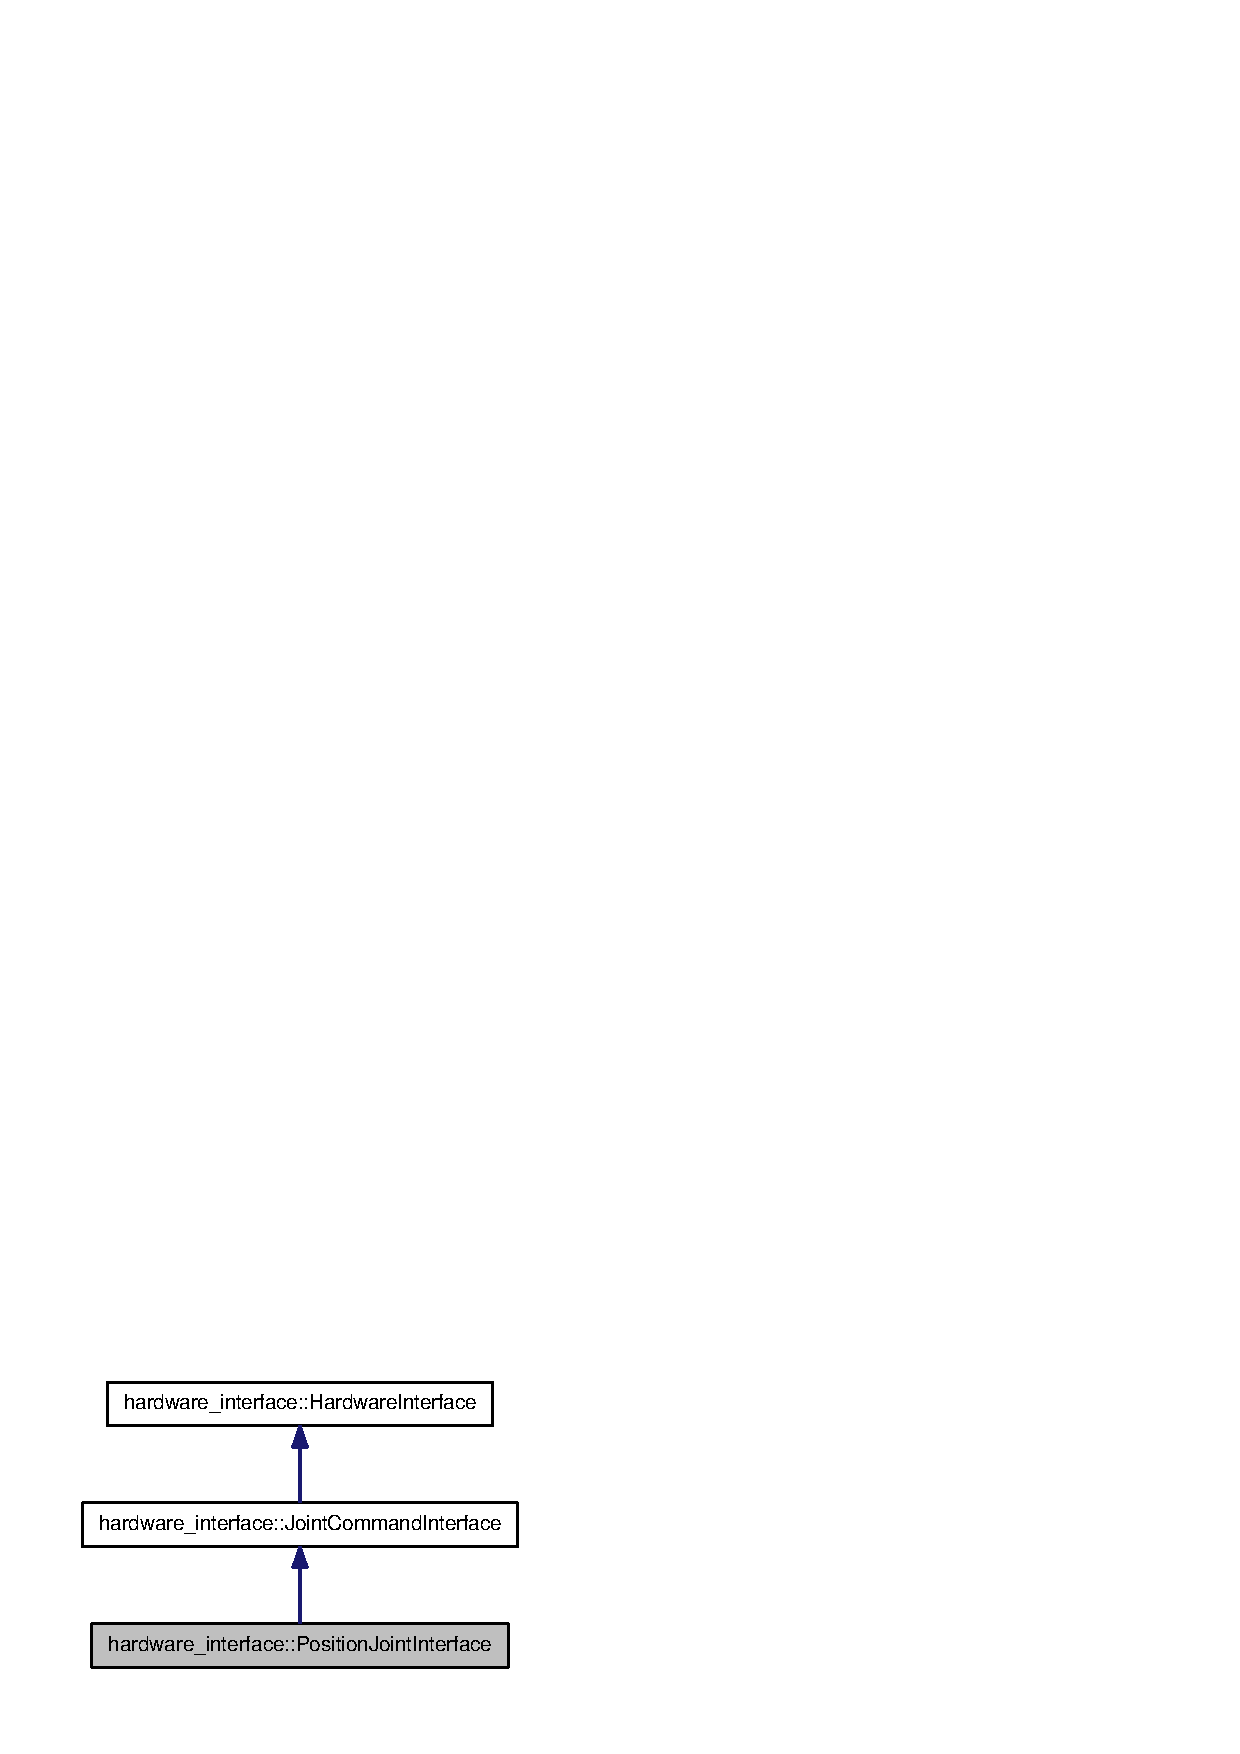
\includegraphics[width=252pt]{classhardware__interface_1_1PositionJointInterface__inherit__graph}
\end{center}
\end{figure}


\subsection{\-Detailed \-Description}
\doxyref{\-Joint\-Command\-Interface}{p.}{classhardware__interface_1_1JointCommandInterface} for commanding position-\/based joints 

\-Definition at line 132 of file joint\-\_\-command\-\_\-interface.\-h.



\-The documentation for this class was generated from the following file\-:\begin{DoxyCompactItemize}
\item 
{\bf joint\-\_\-command\-\_\-interface.\-h}\end{DoxyCompactItemize}

\section{hardware\-\_\-interface\-:\-:\-Robot\-H\-W \-Class \-Reference}
\label{classhardware__interface_1_1RobotHW}\index{hardware\-\_\-interface\-::\-Robot\-H\-W@{hardware\-\_\-interface\-::\-Robot\-H\-W}}


\-Robot \-Hardware \-Interface and \-Resource \-Manager.  




{\ttfamily \#include $<$robot\-\_\-hw.\-h$>$}

\subsection*{\-Public \-Member \-Functions}
\begin{DoxyCompactItemize}
\item 
{\bf \-Robot\-H\-W} ()
\end{DoxyCompactItemize}
\begin{Indent}{\bf \-Resource \-Management}\par
\begin{DoxyCompactItemize}
\item 
virtual bool {\bf check\-For\-Conflict} (const std\-::list$<$ {\bf \-Controller\-Info} $>$ \&info) const 
\end{DoxyCompactItemize}
\end{Indent}
\begin{Indent}{\bf \-Hardware \-Interface \-Management}\par
\begin{DoxyCompactItemize}
\item 
{\footnotesize template$<$class T $>$ }\\void {\bf register\-Interface} (\-T $\ast$hw)
\begin{DoxyCompactList}\small\item\em \-Register a hardware interface. \end{DoxyCompactList}\item 
{\footnotesize template$<$class T $>$ }\\\-T $\ast$ {\bf get} ()
\begin{DoxyCompactList}\small\item\em \-Get a hardware interface. \end{DoxyCompactList}\end{DoxyCompactItemize}
\end{Indent}
\subsection*{\-Private \-Types}
\begin{DoxyCompactItemize}
\item 
typedef std\-::map$<$ std\-::string, \*
{\bf \-Hardware\-Interface} $\ast$ $>$ {\bf \-Interface\-Map}
\end{DoxyCompactItemize}
\subsection*{\-Private \-Attributes}
\begin{DoxyCompactItemize}
\item 
{\bf \-Interface\-Map} {\bf interfaces\-\_\-}
\end{DoxyCompactItemize}


\subsection{\-Detailed \-Description}
\-Robot \-Hardware \-Interface and \-Resource \-Manager. 

\-This class provides a standardized interface to a set of robot hardware interfaces to the controller manager. \-It performs resource conflict checking for a given set of controllers and maintains a map of hardware interfaces. \-It is meant to be used as a base class for abstracting custom robot hardware.

\-The hardware interface map (\doxyref{interfaces\-\_\-}{p.}{classhardware__interface_1_1RobotHW_aff617f06c50fafbe80e95a66df48db1b}) is a 1-\/to-\/1 map between the nams of interface types derived from \doxyref{\-Hardware\-Interface}{p.}{classhardware__interface_1_1HardwareInterface} and instances of those interface types. 

\-Definition at line 53 of file robot\-\_\-hw.\-h.



\subsection{\-Member \-Typedef \-Documentation}
\index{hardware\-\_\-interface\-::\-Robot\-H\-W@{hardware\-\_\-interface\-::\-Robot\-H\-W}!\-Interface\-Map@{\-Interface\-Map}}
\index{\-Interface\-Map@{\-Interface\-Map}!hardware_interface::RobotHW@{hardware\-\_\-interface\-::\-Robot\-H\-W}}
\subsubsection[{\-Interface\-Map}]{\setlength{\rightskip}{0pt plus 5cm}typedef std\-::map$<$std\-::string, {\bf \-Hardware\-Interface}$\ast$$>$ {\bf hardware\-\_\-interface\-::\-Robot\-H\-W\-::\-Interface\-Map}\hspace{0.3cm}{\ttfamily  [private]}}\label{classhardware__interface_1_1RobotHW_a3272b83ff82468de130926610cc1b9bc}


\-Definition at line 145 of file robot\-\_\-hw.\-h.



\subsection{\-Constructor \& \-Destructor \-Documentation}
\index{hardware\-\_\-interface\-::\-Robot\-H\-W@{hardware\-\_\-interface\-::\-Robot\-H\-W}!\-Robot\-H\-W@{\-Robot\-H\-W}}
\index{\-Robot\-H\-W@{\-Robot\-H\-W}!hardware_interface::RobotHW@{hardware\-\_\-interface\-::\-Robot\-H\-W}}
\subsubsection[{\-Robot\-H\-W}]{\setlength{\rightskip}{0pt plus 5cm}{\bf hardware\-\_\-interface\-::\-Robot\-H\-W\-::\-Robot\-H\-W} (
\begin{DoxyParamCaption}
{}
\end{DoxyParamCaption}
)\hspace{0.3cm}{\ttfamily  [inline]}}\label{classhardware__interface_1_1RobotHW_ade9bd05d3157dc2d278bcb2d19d6b6e6}


\-Definition at line 56 of file robot\-\_\-hw.\-h.



\subsection{\-Member \-Function \-Documentation}
\index{hardware\-\_\-interface\-::\-Robot\-H\-W@{hardware\-\_\-interface\-::\-Robot\-H\-W}!check\-For\-Conflict@{check\-For\-Conflict}}
\index{check\-For\-Conflict@{check\-For\-Conflict}!hardware_interface::RobotHW@{hardware\-\_\-interface\-::\-Robot\-H\-W}}
\subsubsection[{check\-For\-Conflict}]{\setlength{\rightskip}{0pt plus 5cm}virtual bool {\bf hardware\-\_\-interface\-::\-Robot\-H\-W\-::check\-For\-Conflict} (
\begin{DoxyParamCaption}
\item[{const std\-::list$<$ {\bf \-Controller\-Info} $>$ \&}]{info}
\end{DoxyParamCaption}
) const\hspace{0.3cm}{\ttfamily  [inline, virtual]}}\label{classhardware__interface_1_1RobotHW_a96a73831d8e36a746102752383feec61}
\-Check (in non-\/realtime) if the given set of controllers is allowed to run simultaneously.

\-This default implementation simply checks if any two controllers use the same resource. 

\-Definition at line 70 of file robot\-\_\-hw.\-h.

\index{hardware\-\_\-interface\-::\-Robot\-H\-W@{hardware\-\_\-interface\-::\-Robot\-H\-W}!get@{get}}
\index{get@{get}!hardware_interface::RobotHW@{hardware\-\_\-interface\-::\-Robot\-H\-W}}
\subsubsection[{get}]{\setlength{\rightskip}{0pt plus 5cm}template$<$class T $>$ \-T$\ast$ {\bf hardware\-\_\-interface\-::\-Robot\-H\-W\-::get} (
\begin{DoxyParamCaption}
{}
\end{DoxyParamCaption}
)\hspace{0.3cm}{\ttfamily  [inline]}}\label{classhardware__interface_1_1RobotHW_a75dc7e362f3c2905606809d414d953c1}


\-Get a hardware interface. 

\-Since \doxyref{\-Robot\-H\-W}{p.}{classhardware__interface_1_1RobotHW} only stores one interface per type, this returns a pointer to the requested interface type. \-If the interface type is not registered, it will return {\ttfamily \-N\-U\-L\-L}.


\begin{DoxyTemplParams}{\-Template Parameters}
{\em \-T} & \-The hardware interface type \\
\hline
\end{DoxyTemplParams}
\begin{DoxyReturn}{\-Returns}
\-A pointer to a hardware interface or {\ttfamily \-N\-U\-L\-L} 
\end{DoxyReturn}


\-Definition at line 127 of file robot\-\_\-hw.\-h.

\index{hardware\-\_\-interface\-::\-Robot\-H\-W@{hardware\-\_\-interface\-::\-Robot\-H\-W}!register\-Interface@{register\-Interface}}
\index{register\-Interface@{register\-Interface}!hardware_interface::RobotHW@{hardware\-\_\-interface\-::\-Robot\-H\-W}}
\subsubsection[{register\-Interface}]{\setlength{\rightskip}{0pt plus 5cm}template$<$class T $>$ void {\bf hardware\-\_\-interface\-::\-Robot\-H\-W\-::register\-Interface} (
\begin{DoxyParamCaption}
\item[{\-T $\ast$}]{hw}
\end{DoxyParamCaption}
)\hspace{0.3cm}{\ttfamily  [inline]}}\label{classhardware__interface_1_1RobotHW_a9f418188d3552ce303fa4184d212e788}


\-Register a hardware interface. 

\-This associates the name of the type of interface to be registered with the given pointer.


\begin{DoxyTemplParams}{\-Template Parameters}
{\em \-T} & \-The hardware interface type \\
\hline
\end{DoxyTemplParams}

\begin{DoxyParams}{\-Parameters}
{\em hw} & \-A pointer to a hardware interface \\
\hline
\end{DoxyParams}


\-Definition at line 110 of file robot\-\_\-hw.\-h.



\subsection{\-Member \-Data \-Documentation}
\index{hardware\-\_\-interface\-::\-Robot\-H\-W@{hardware\-\_\-interface\-::\-Robot\-H\-W}!interfaces\-\_\-@{interfaces\-\_\-}}
\index{interfaces\-\_\-@{interfaces\-\_\-}!hardware_interface::RobotHW@{hardware\-\_\-interface\-::\-Robot\-H\-W}}
\subsubsection[{interfaces\-\_\-}]{\setlength{\rightskip}{0pt plus 5cm}{\bf \-Interface\-Map} {\bf hardware\-\_\-interface\-::\-Robot\-H\-W\-::interfaces\-\_\-}\hspace{0.3cm}{\ttfamily  [private]}}\label{classhardware__interface_1_1RobotHW_aff617f06c50fafbe80e95a66df48db1b}


\-Definition at line 146 of file robot\-\_\-hw.\-h.



\-The documentation for this class was generated from the following file\-:\begin{DoxyCompactItemize}
\item 
{\bf robot\-\_\-hw.\-h}\end{DoxyCompactItemize}

\section{hardware\-\_\-interface\-:\-:\-Velocity\-Joint\-Interface \-Class \-Reference}
\label{classhardware__interface_1_1VelocityJointInterface}\index{hardware\-\_\-interface\-::\-Velocity\-Joint\-Interface@{hardware\-\_\-interface\-::\-Velocity\-Joint\-Interface}}


\doxyref{\-Joint\-Command\-Interface}{p.}{classhardware__interface_1_1JointCommandInterface} for commanding velocity-\/based joints  




{\ttfamily \#include $<$joint\-\_\-command\-\_\-interface.\-h$>$}



\-Inheritance diagram for hardware\-\_\-interface\-:\-:\-Velocity\-Joint\-Interface\-:
\nopagebreak
\begin{figure}[H]
\begin{center}
\leavevmode
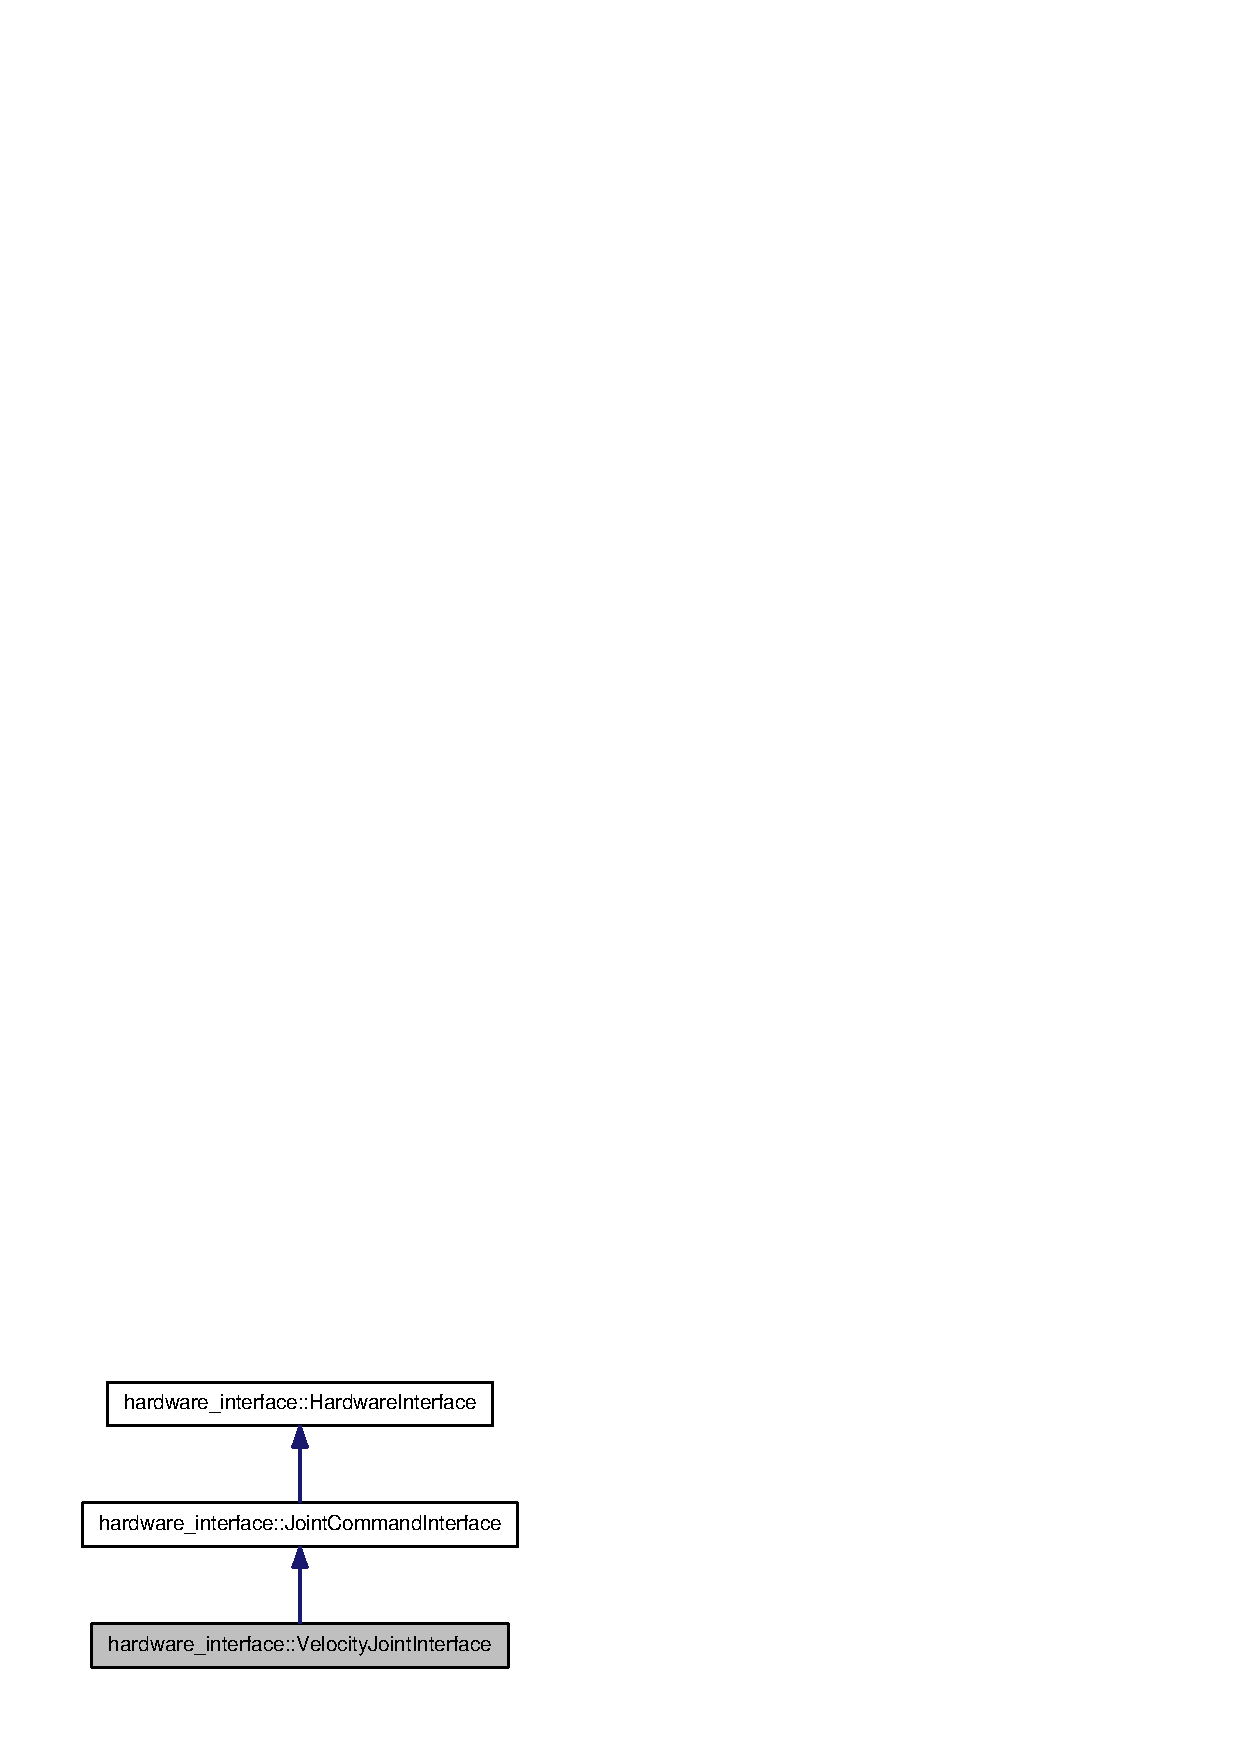
\includegraphics[width=252pt]{classhardware__interface_1_1VelocityJointInterface__inherit__graph}
\end{center}
\end{figure}


\subsection{\-Detailed \-Description}
\doxyref{\-Joint\-Command\-Interface}{p.}{classhardware__interface_1_1JointCommandInterface} for commanding velocity-\/based joints 

\-Definition at line 126 of file joint\-\_\-command\-\_\-interface.\-h.



\-The documentation for this class was generated from the following file\-:\begin{DoxyCompactItemize}
\item 
{\bf joint\-\_\-command\-\_\-interface.\-h}\end{DoxyCompactItemize}

\chapter{\-File \-Documentation}
\section{controller\-\_\-info.\-h \-File \-Reference}
\label{controller__info_8h}\index{controller\-\_\-info.\-h@{controller\-\_\-info.\-h}}
{\ttfamily \#include $<$set$>$}\*
{\ttfamily \#include $<$string$>$}\*
\-Include dependency graph for controller\-\_\-info.\-h\-:
\nopagebreak
\begin{figure}[H]
\begin{center}
\leavevmode
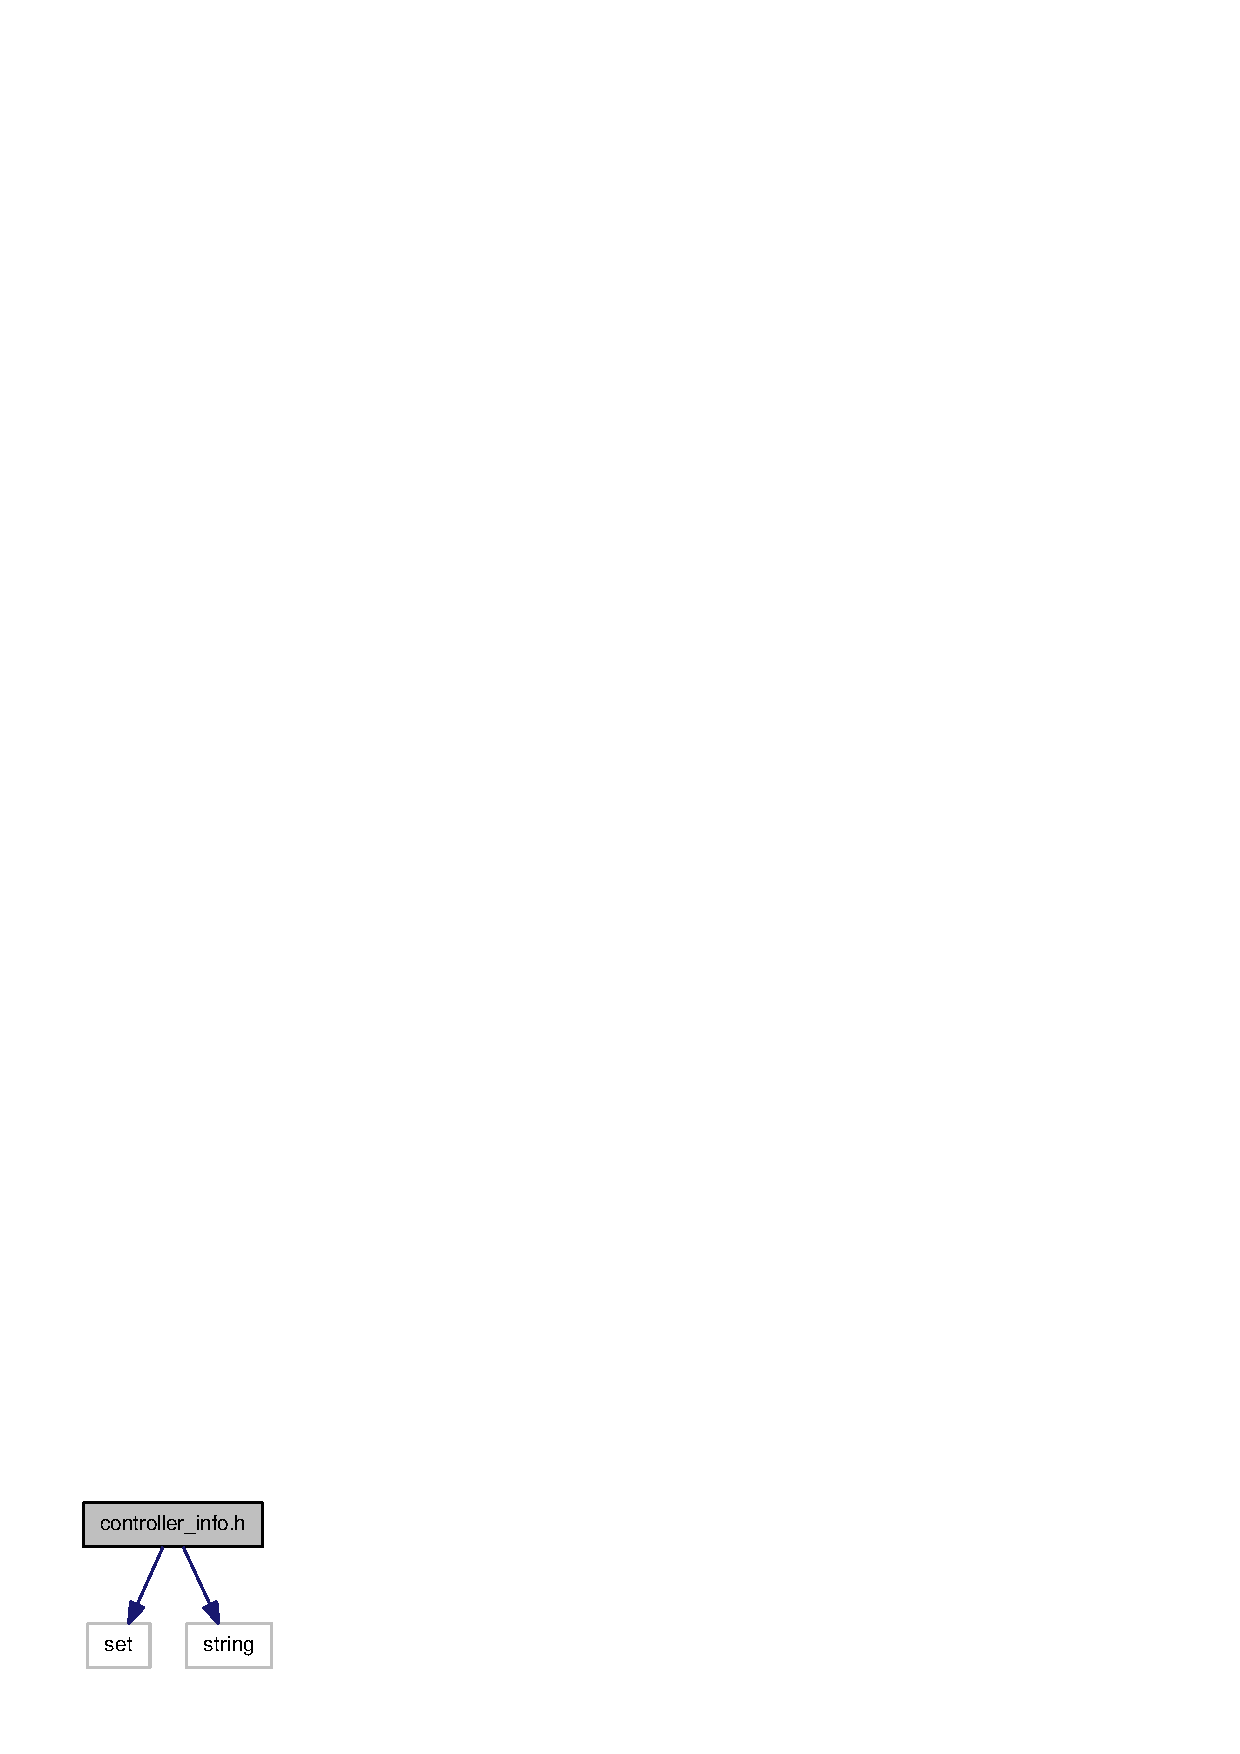
\includegraphics[width=134pt]{controller__info_8h__incl}
\end{center}
\end{figure}
\-This graph shows which files directly or indirectly include this file\-:
\nopagebreak
\begin{figure}[H]
\begin{center}
\leavevmode
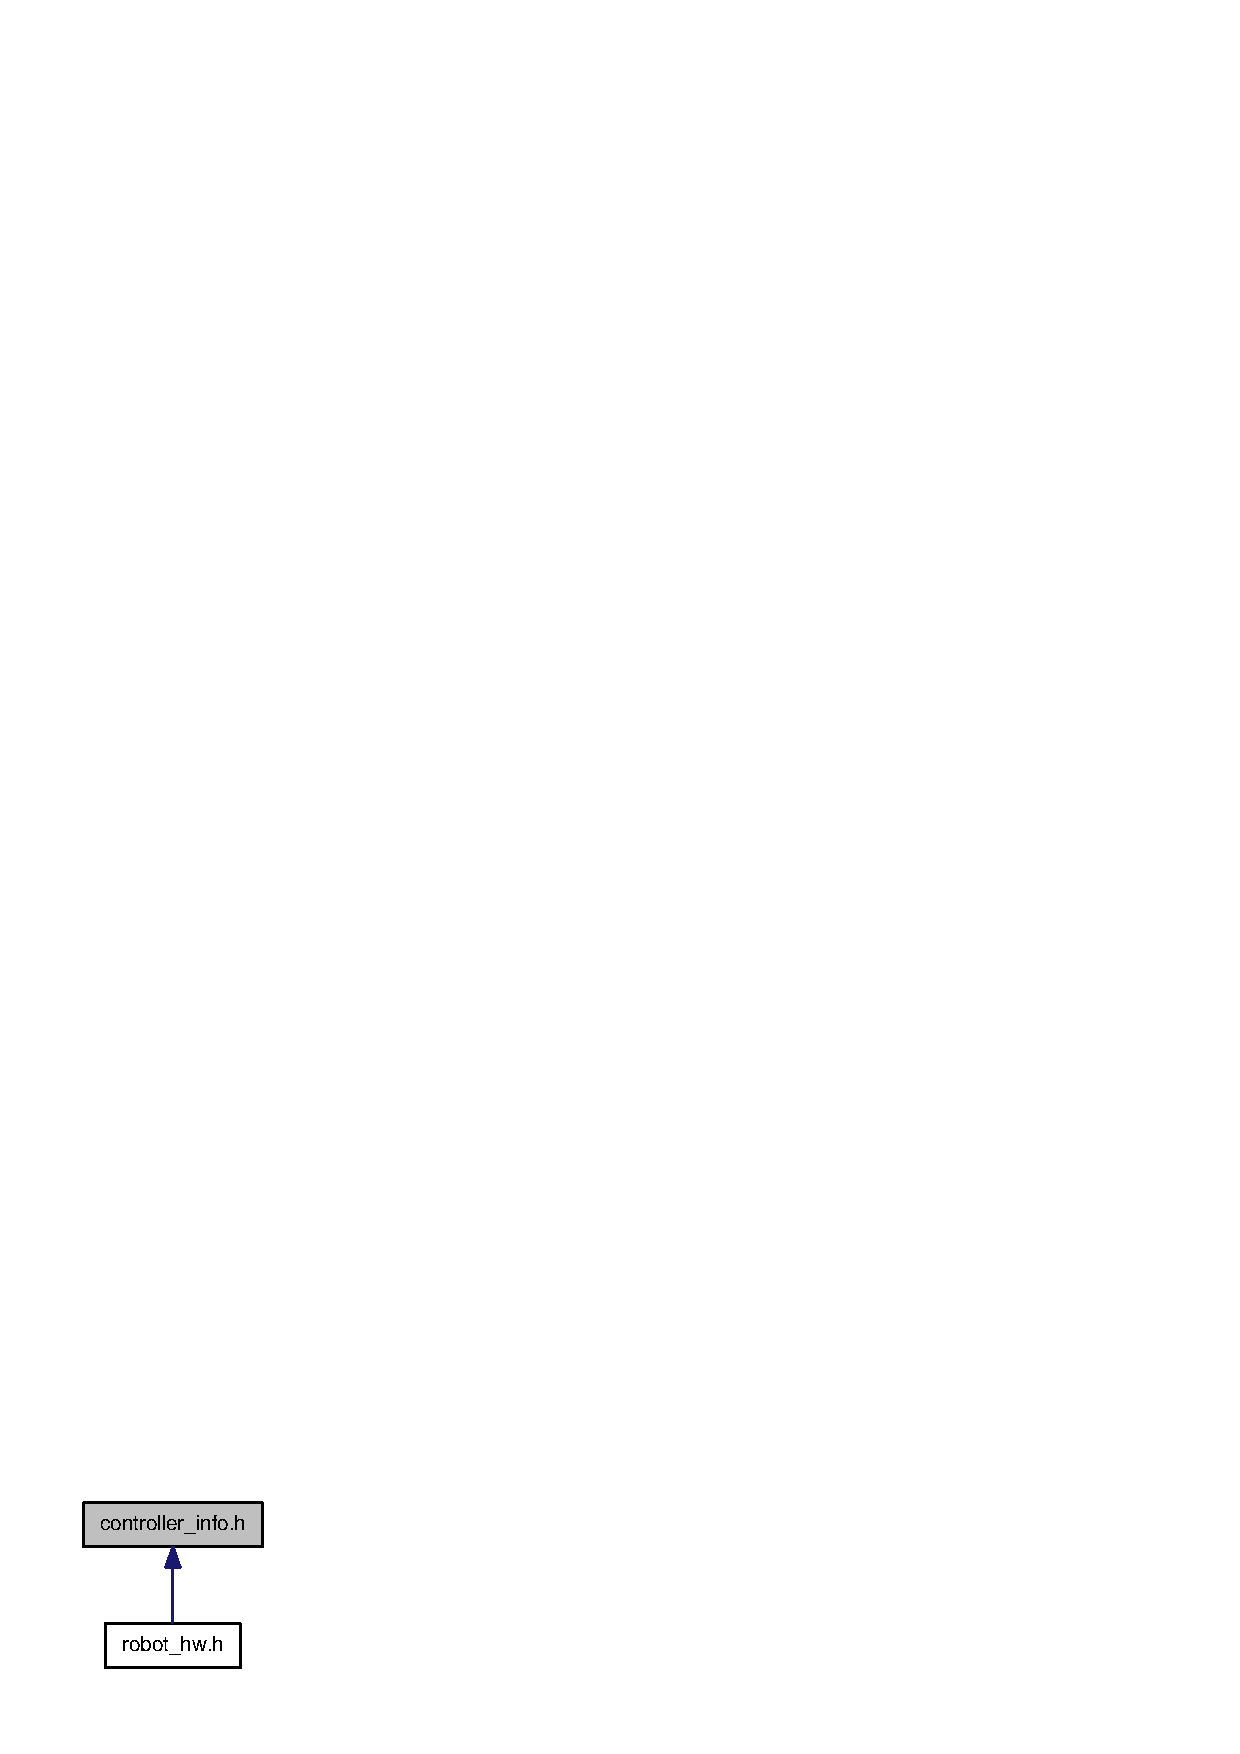
\includegraphics[width=130pt]{controller__info_8h__dep__incl}
\end{center}
\end{figure}
\subsection*{\-Classes}
\begin{DoxyCompactItemize}
\item 
struct {\bf hardware\-\_\-interface\-::\-Controller\-Info}
\begin{DoxyCompactList}\small\item\em \-Controller \-Information. \end{DoxyCompactList}\end{DoxyCompactItemize}
\subsection*{\-Namespaces}
\begin{DoxyCompactItemize}
\item 
namespace {\bf hardware\-\_\-interface}
\end{DoxyCompactItemize}

\section{hardware\-\_\-interface.\-h \-File \-Reference}
\label{hardware__interface_8h}\index{hardware\-\_\-interface.\-h@{hardware\-\_\-interface.\-h}}
{\ttfamily \#include $<$exception$>$}\*
{\ttfamily \#include $<$string$>$}\*
{\ttfamily \#include $<$set$>$}\*
{\ttfamily \#include $<$typeinfo$>$}\*
\-Include dependency graph for hardware\-\_\-interface.\-h\-:
\nopagebreak
\begin{figure}[H]
\begin{center}
\leavevmode
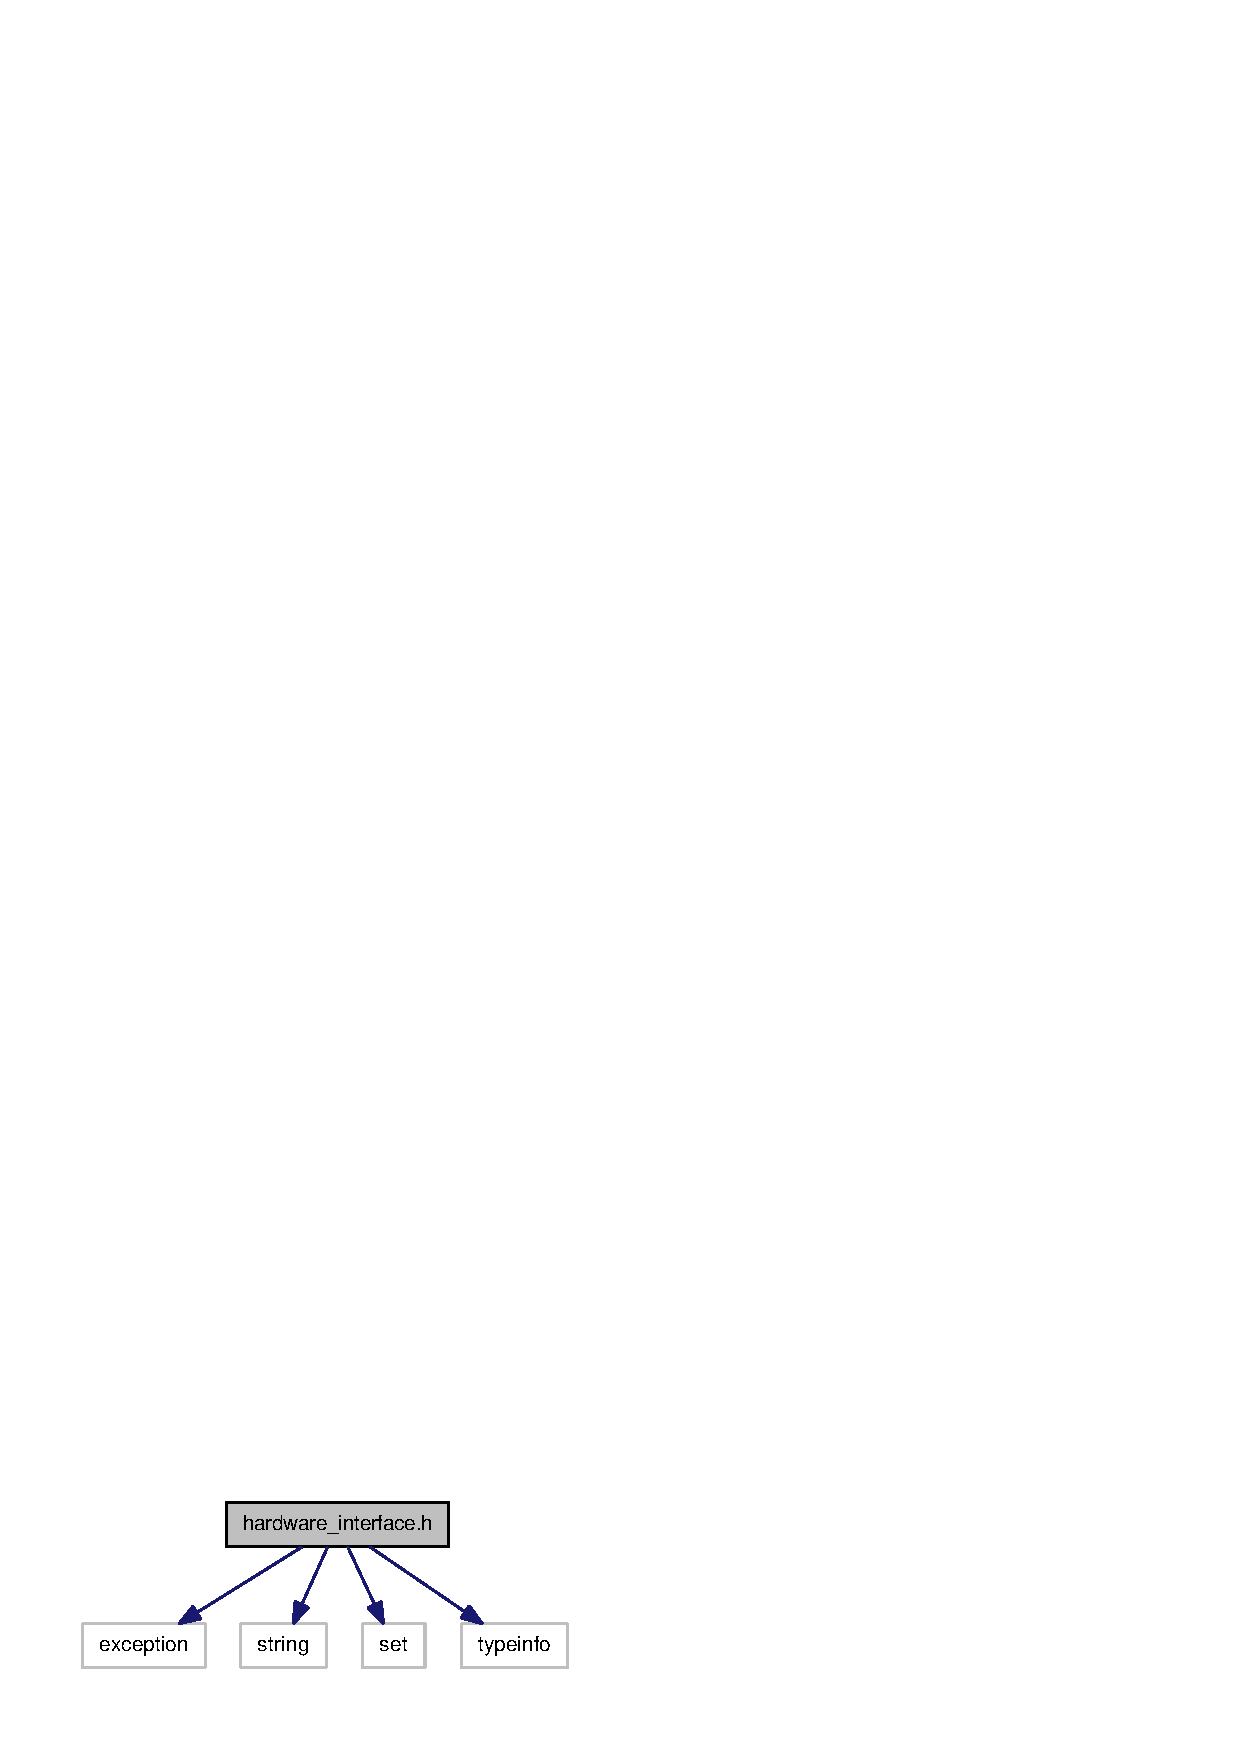
\includegraphics[width=276pt]{hardware__interface_8h__incl}
\end{center}
\end{figure}
\-This graph shows which files directly or indirectly include this file\-:
\nopagebreak
\begin{figure}[H]
\begin{center}
\leavevmode
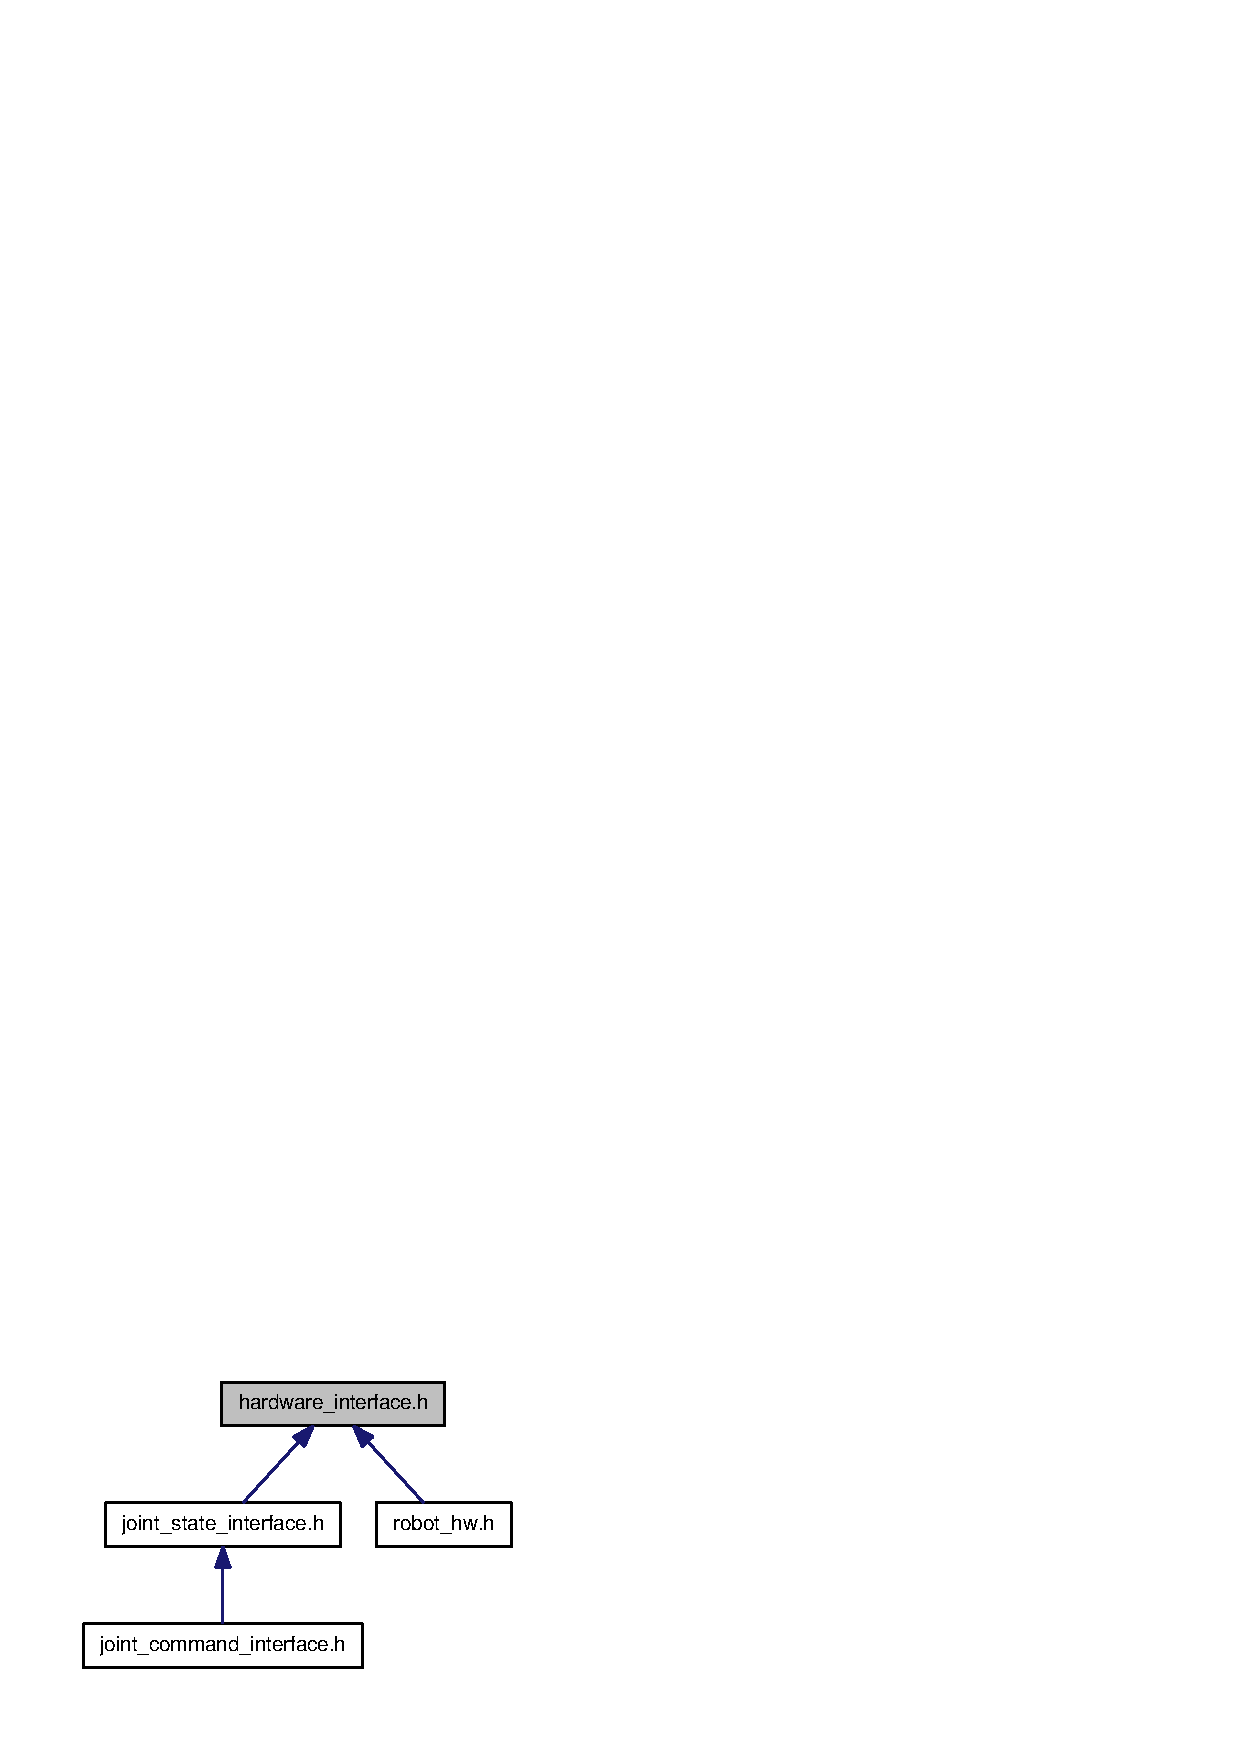
\includegraphics[width=249pt]{hardware__interface_8h__dep__incl}
\end{center}
\end{figure}
\subsection*{\-Classes}
\begin{DoxyCompactItemize}
\item 
class {\bf hardware\-\_\-interface\-::\-Hardware\-Interface}
\begin{DoxyCompactList}\small\item\em \-Abstract \-Hardware \-Interface. \end{DoxyCompactList}\item 
class {\bf hardware\-\_\-interface\-::\-Hardware\-Interface\-Exception}
\begin{DoxyCompactList}\small\item\em \-An exception related to a \doxyref{\-Hardware\-Interface}{p.}{classhardware__interface_1_1HardwareInterface}. \end{DoxyCompactList}\end{DoxyCompactItemize}
\subsection*{\-Namespaces}
\begin{DoxyCompactItemize}
\item 
namespace {\bf hardware\-\_\-interface}
\end{DoxyCompactItemize}

\section{joint\-\_\-command\-\_\-interface.\-h \-File \-Reference}
\label{joint__command__interface_8h}\index{joint\-\_\-command\-\_\-interface.\-h@{joint\-\_\-command\-\_\-interface.\-h}}
{\ttfamily \#include $<$hardware\-\_\-interface/joint\-\_\-state\-\_\-interface.\-h$>$}\*
\-Include dependency graph for joint\-\_\-command\-\_\-interface.\-h\-:
\nopagebreak
\begin{figure}[H]
\begin{center}
\leavevmode
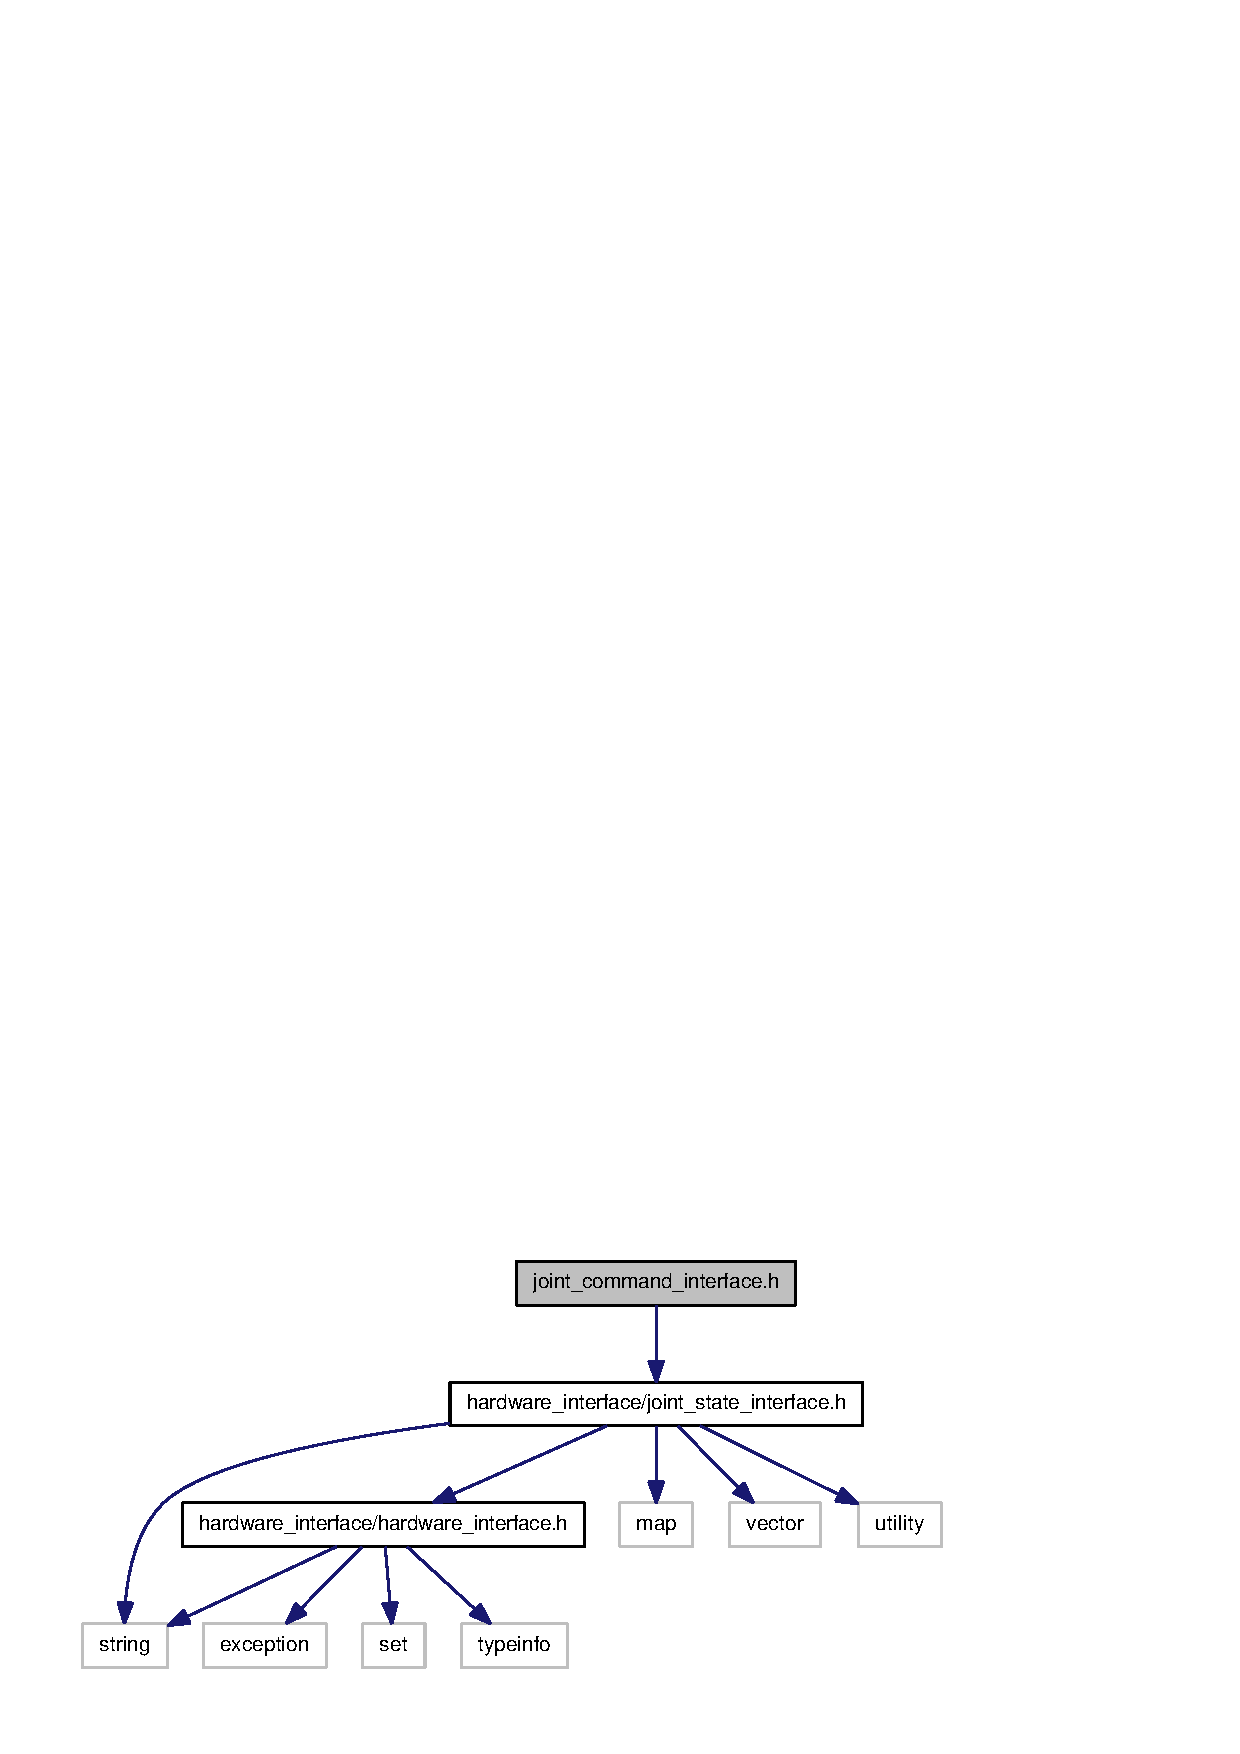
\includegraphics[width=350pt]{joint__command__interface_8h__incl}
\end{center}
\end{figure}
\subsection*{\-Classes}
\begin{DoxyCompactItemize}
\item 
class {\bf hardware\-\_\-interface\-::\-Effort\-Joint\-Interface}
\begin{DoxyCompactList}\small\item\em \doxyref{\-Joint\-Command\-Interface}{p.}{classhardware__interface_1_1JointCommandInterface} for commanding effort-\/based joints \end{DoxyCompactList}\item 
class {\bf hardware\-\_\-interface\-::\-Joint\-Command\-Interface}
\begin{DoxyCompactList}\small\item\em \-Hardware interface to support commanding an array of joints. \end{DoxyCompactList}\item 
class {\bf hardware\-\_\-interface\-::\-Joint\-Handle}
\begin{DoxyCompactList}\small\item\em \-A handle used to read and command a single joint. \end{DoxyCompactList}\item 
class {\bf hardware\-\_\-interface\-::\-Position\-Joint\-Interface}
\begin{DoxyCompactList}\small\item\em \doxyref{\-Joint\-Command\-Interface}{p.}{classhardware__interface_1_1JointCommandInterface} for commanding position-\/based joints \end{DoxyCompactList}\item 
class {\bf hardware\-\_\-interface\-::\-Velocity\-Joint\-Interface}
\begin{DoxyCompactList}\small\item\em \doxyref{\-Joint\-Command\-Interface}{p.}{classhardware__interface_1_1JointCommandInterface} for commanding velocity-\/based joints \end{DoxyCompactList}\end{DoxyCompactItemize}
\subsection*{\-Namespaces}
\begin{DoxyCompactItemize}
\item 
namespace {\bf hardware\-\_\-interface}
\end{DoxyCompactItemize}

\section{joint\-\_\-state\-\_\-interface.\-h \-File \-Reference}
\label{joint__state__interface_8h}\index{joint\-\_\-state\-\_\-interface.\-h@{joint\-\_\-state\-\_\-interface.\-h}}
{\ttfamily \#include $<$hardware\-\_\-interface/hardware\-\_\-interface.\-h$>$}\*
{\ttfamily \#include $<$string$>$}\*
{\ttfamily \#include $<$map$>$}\*
{\ttfamily \#include $<$vector$>$}\*
{\ttfamily \#include $<$utility$>$}\*
\-Include dependency graph for joint\-\_\-state\-\_\-interface.\-h\-:
\nopagebreak
\begin{figure}[H]
\begin{center}
\leavevmode
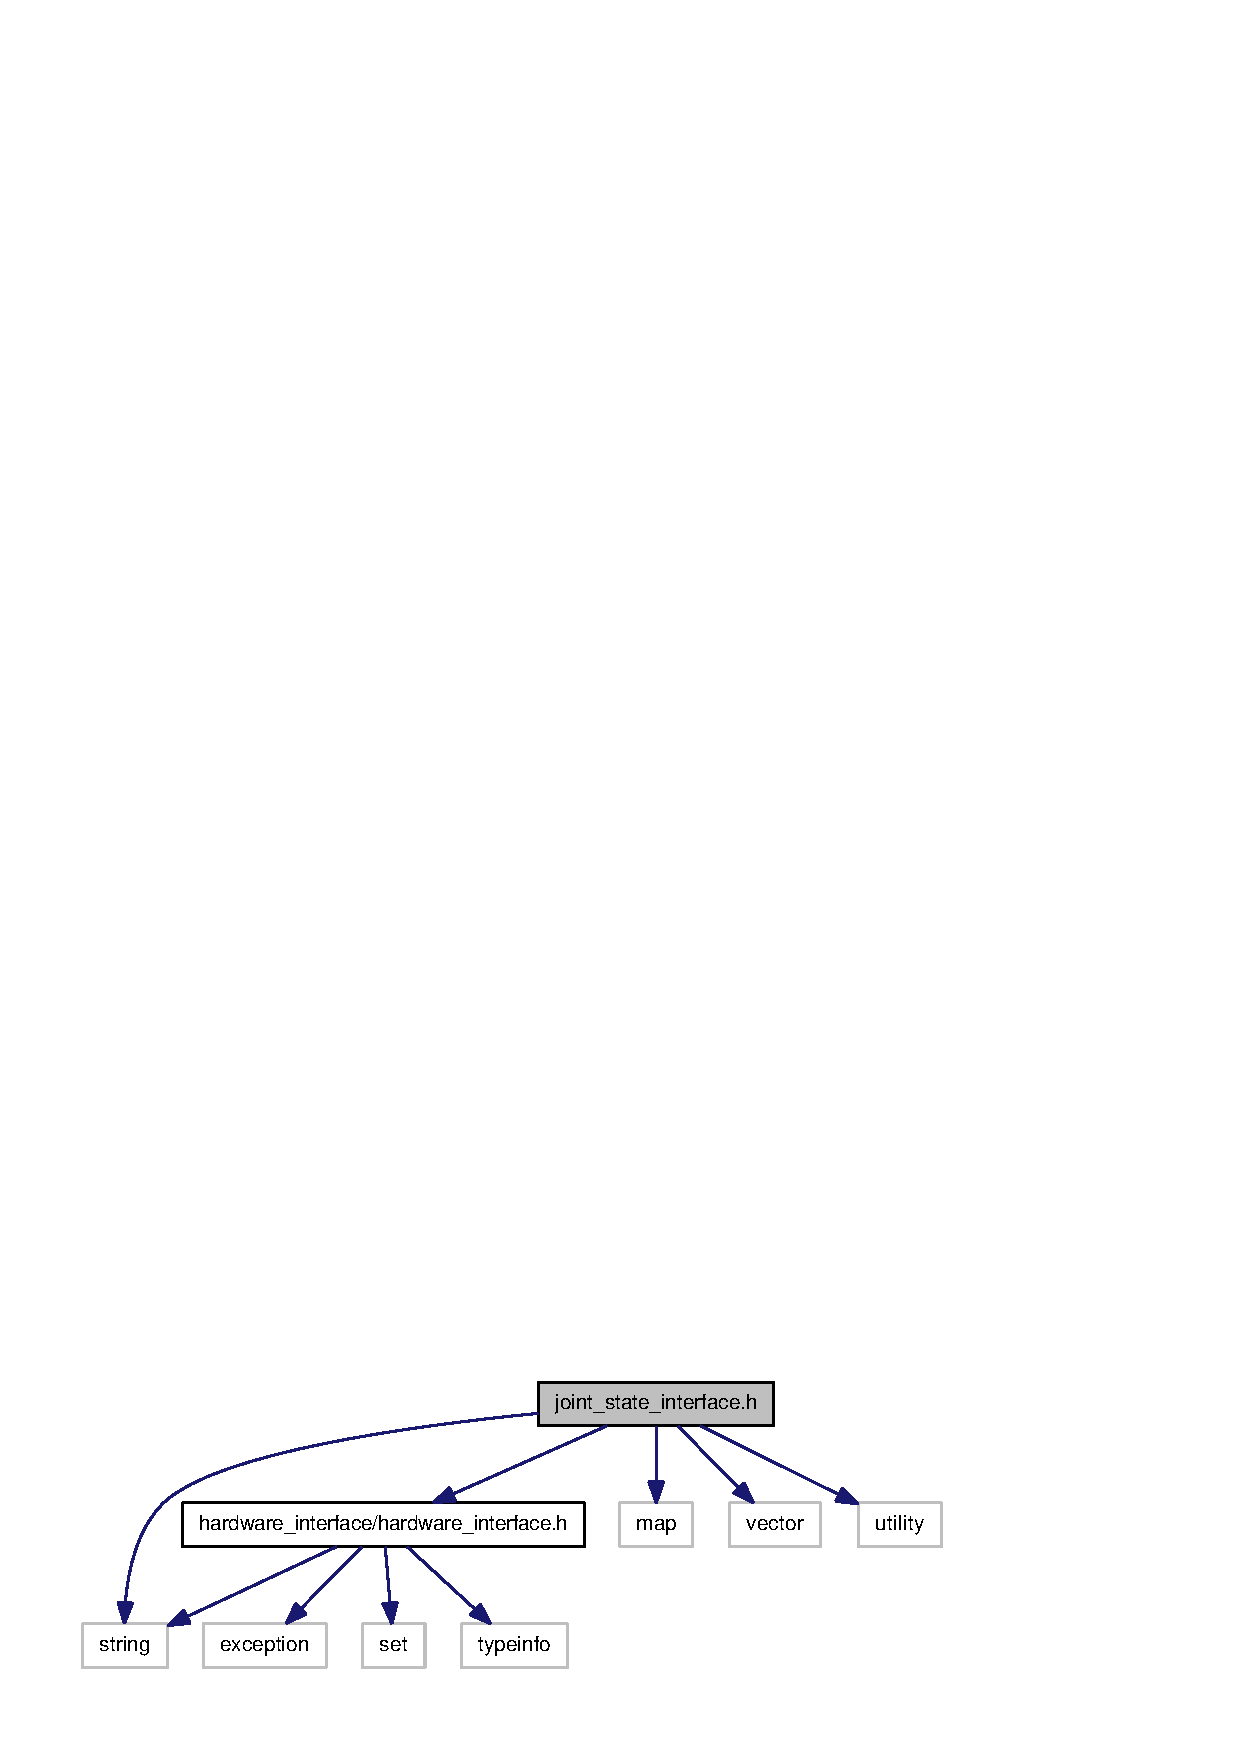
\includegraphics[width=350pt]{joint__state__interface_8h__incl}
\end{center}
\end{figure}
\-This graph shows which files directly or indirectly include this file\-:
\nopagebreak
\begin{figure}[H]
\begin{center}
\leavevmode
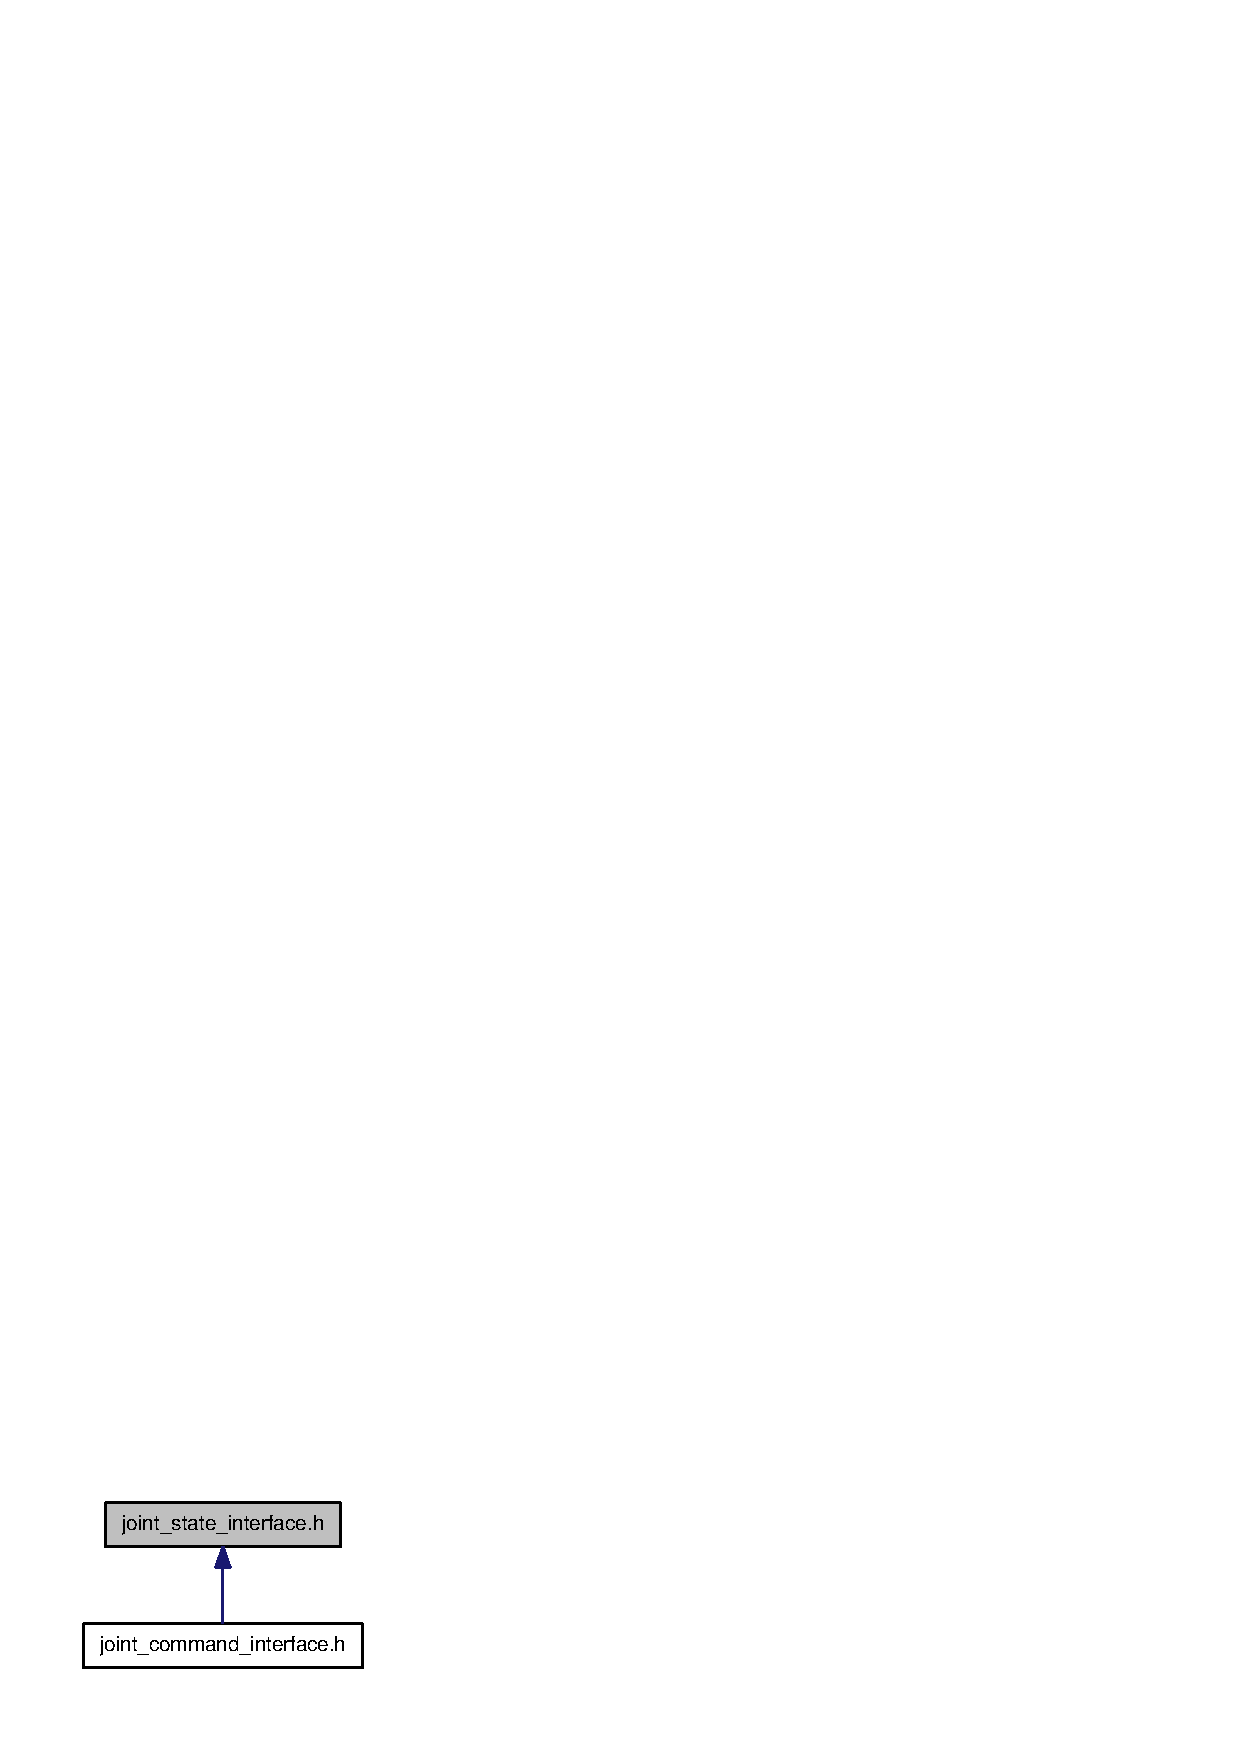
\includegraphics[width=178pt]{joint__state__interface_8h__dep__incl}
\end{center}
\end{figure}
\subsection*{\-Classes}
\begin{DoxyCompactItemize}
\item 
class {\bf hardware\-\_\-interface\-::\-Joint\-State\-Handle}
\begin{DoxyCompactList}\small\item\em \-A handle used to read the state of a single joint. \end{DoxyCompactList}\item 
class {\bf hardware\-\_\-interface\-::\-Joint\-State\-Interface}
\begin{DoxyCompactList}\small\item\em \-Hardware interface to support reading the state of an array of joints. \end{DoxyCompactList}\end{DoxyCompactItemize}
\subsection*{\-Namespaces}
\begin{DoxyCompactItemize}
\item 
namespace {\bf hardware\-\_\-interface}
\end{DoxyCompactItemize}

\section{robot\-\_\-hw.\-h \-File \-Reference}
\label{robot__hw_8h}\index{robot\-\_\-hw.\-h@{robot\-\_\-hw.\-h}}
{\ttfamily \#include $<$map$>$}\*
{\ttfamily \#include $<$typeinfo$>$}\*
{\ttfamily \#include $<$hardware\-\_\-interface/hardware\-\_\-interface.\-h$>$}\*
{\ttfamily \#include $<$hardware\-\_\-interface/controller\-\_\-info.\-h$>$}\*
{\ttfamily \#include $<$ros/ros.\-h$>$}\*
\-Include dependency graph for robot\-\_\-hw.\-h\-:
\nopagebreak
\begin{figure}[H]
\begin{center}
\leavevmode
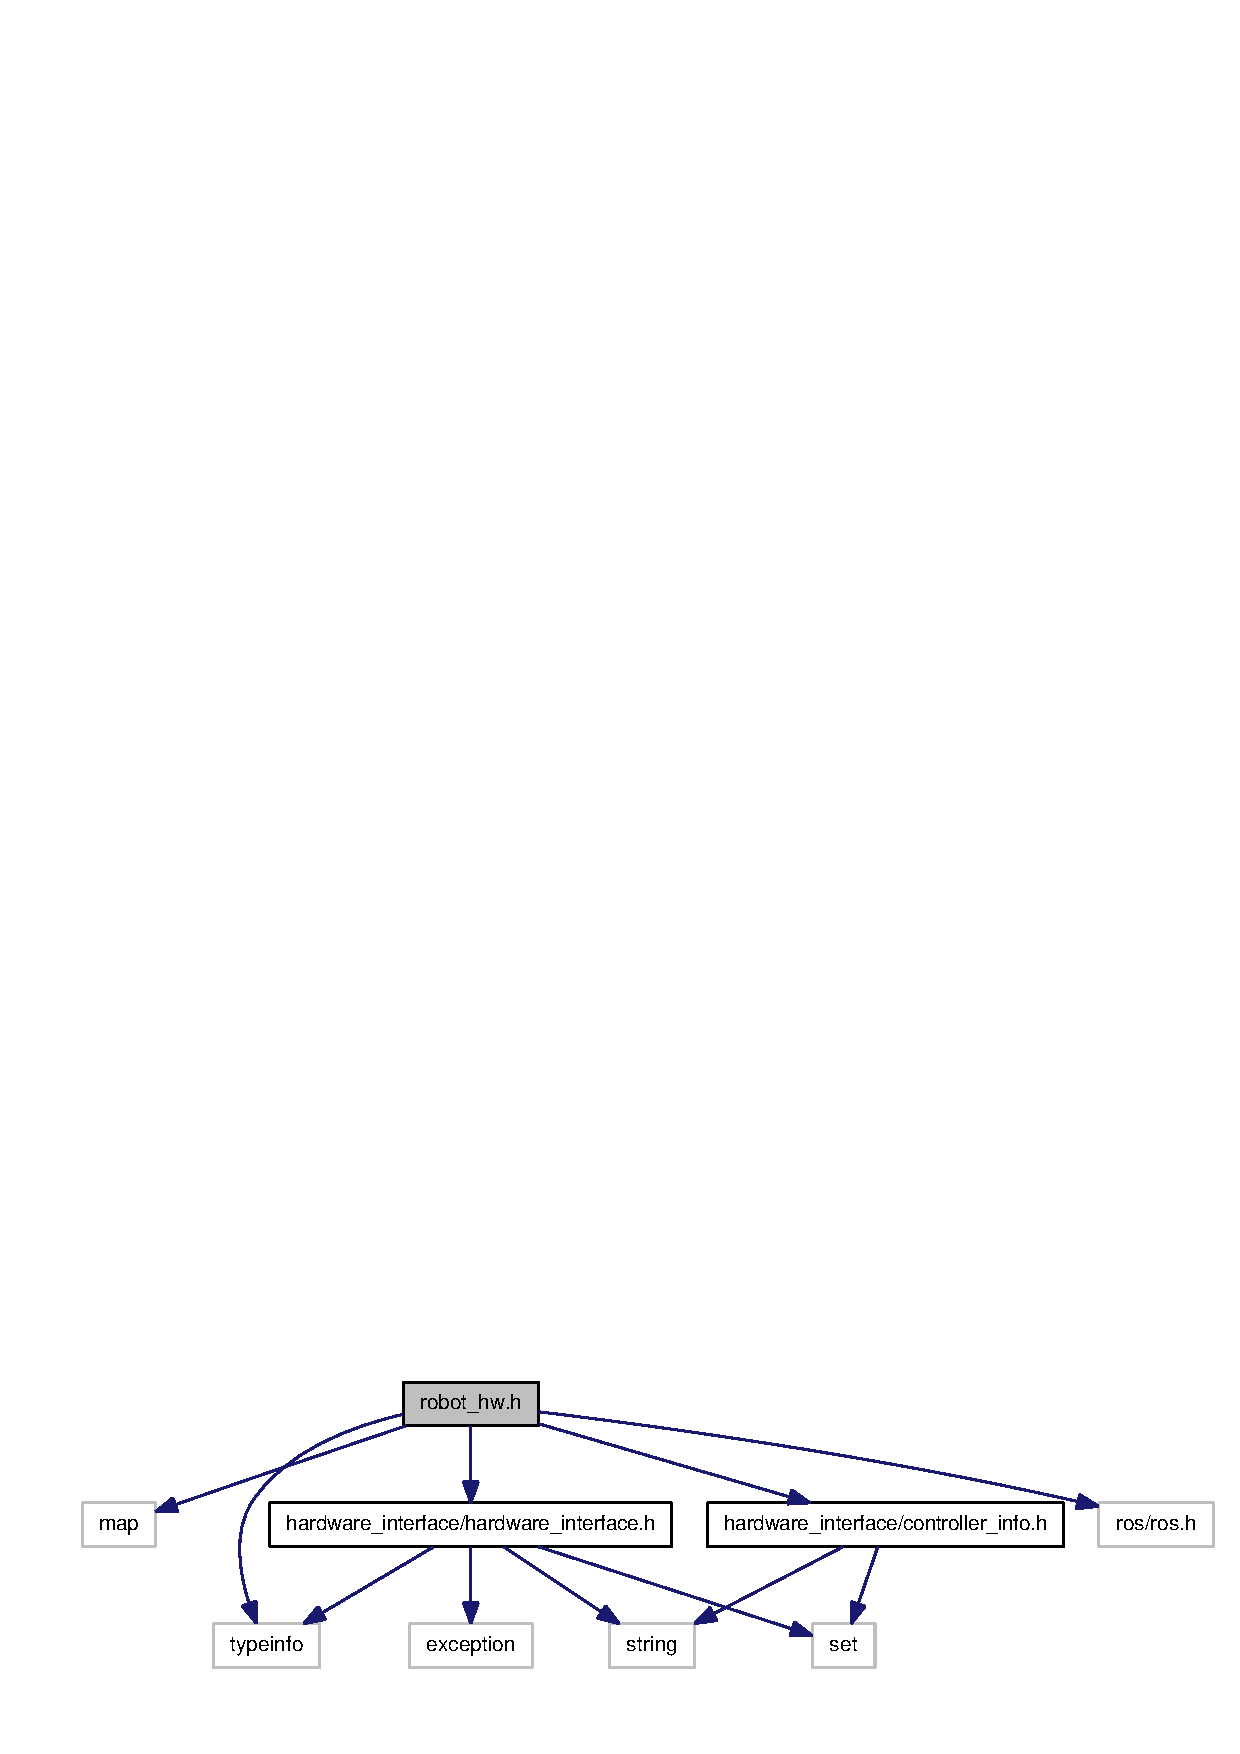
\includegraphics[width=350pt]{robot__hw_8h__incl}
\end{center}
\end{figure}
\subsection*{\-Classes}
\begin{DoxyCompactItemize}
\item 
class {\bf hardware\-\_\-interface\-::\-Robot\-H\-W}
\begin{DoxyCompactList}\small\item\em \-Robot \-Hardware \-Interface and \-Resource \-Manager. \end{DoxyCompactList}\end{DoxyCompactItemize}
\subsection*{\-Namespaces}
\begin{DoxyCompactItemize}
\item 
namespace {\bf hardware\-\_\-interface}
\end{DoxyCompactItemize}

\printindex
\end{document}
